\documentclass[10pt,letterpaper]{article}
\usepackage[utf8]{inputenc}
\usepackage[T1]{fontenc}
\usepackage{lmodern}
\usepackage[letterpaper,top=2.0cm,bottom=2.0cm,left=2.0cm,right=2.0cm]{geometry}
\usepackage{amsmath,amssymb}
\usepackage{booktabs}
\usepackage{tabularx}
\usepackage{xltabular}
\usepackage{pdflscape}
\usepackage{colortbl}
\usepackage{microtype}
\usepackage{array}
\usepackage{xcolor}
\usepackage{graphicx}
\graphicspath{{figuras/}{./}}
\usepackage{float}
\usepackage{fancyhdr}
\usepackage{tcolorbox}
\tcbuselibrary{skins,breakable}
\usepackage{hyperref}
\usepackage{titlesec}
\usepackage{enumitem}
\usepackage{lastpage}
\usepackage{caption}
\usepackage{pdfpages}

\renewcommand{\contentsname}{Índice General}
\renewcommand{\listtablename}{Índice de Cuadros}
\renewcommand{\listfigurename}{Índice de Figuras}
\captionsetup[table]{name=Cuadro,labelfont=bf,textfont=bf,skip=4pt}
\captionsetup[figure]{name=Figura,labelfont=bf,textfont=bf,skip=4pt}

\setlist{nosep,leftmargin=1.3em}
\setlength{\parindent}{0pt}
\setlength{\parskip}{3.5pt}

\definecolor{navyblue}{RGB}{26, 79, 124}
\definecolor{accentblue}{RGB}{51, 124, 207}
\definecolor{darkred}{RGB}{140, 30, 30}
\definecolor{tealcolor}{RGB}{30, 110, 110}
\definecolor{forestgreen}{RGB}{20, 120, 40}
\definecolor{boxbg}{RGB}{250, 251, 253}
\definecolor{tableheader}{RGB}{26, 79, 124}
\definecolor{tablerowalt}{RGB}{245, 248, 252}
\definecolor{grayborder}{RGB}{208, 215, 222}

\titleformat{\section}{\large\bfseries\color{navyblue}}{\thesection.}{0.5em}{}
\titleformat{\subsection}{\normalsize\bfseries\color{navyblue}}{\thesubsection.}{0.5em}{}
\titleformat{\subsubsection}{\small\bfseries\color{accentblue}}{\thesubsubsection.}{0.5em}{}
\titlespacing*{\section}{0pt}{5pt}{2pt}
\titlespacing*{\subsection}{0pt}{4pt}{1pt}
\titlespacing*{\subsubsection}{0pt}{3pt}{1pt}

\pagestyle{fancy}
\fancyhf{}
\lhead{\small\color{navyblue}\textbf{Solvanta Engineering Solutions} \textbar\ DPyPQ}
\rhead{\small AC-HAZOP-01 \textbar\ Expediente Técnico HAZOP y MCE-01 Rev. 1}
\cfoot{\small Página \thepage\ de \pageref{LastPage}}
\renewcommand{\headrulewidth}{0.4pt}
\renewcommand{\footrulewidth}{0pt}
\setlength{\headheight}{14pt}

\hypersetup{
    colorlinks=true,
    linkcolor=navyblue,
    citecolor=navyblue,
    urlcolor=accentblue,
    pdfauthor={Solvanta Engineering Solutions S.A. de C.V.},
    pdftitle={AC-HAZOP-01: Expediente HAZOP, MCE-01 Rev. 1 y Trazabilidad DTI v1}
}

\begin{document}

% --- PORTADA CORPORATIVA OFICIAL ---
\begin{titlepage}
    \centering
    
\includegraphics[width=0.28\textwidth]{figuras/logo_empresa.png}\\[0.3cm]
    {\scshape\Large Benemérita Universidad Autónoma de Puebla}\\[0.1cm]
    {\scshape\large Facultad de Ingeniería Química \textbar\ Colegio de Ingeniería Química}\\[0.1cm]
    {\large Diseño de Procesos y Productos Químicos (DPyPQ)}\\[0.1cm]
    {\small Catedrático: Dr. Jesús Andrés Arzola Flores}\\[0.4cm]
    \hrule height 2pt
    \vspace{0.3cm}
    {\LARGE \bfseries \color{navyblue} ACTIVIDAD INTEGRADORA AC-HAZOP-01\par}
    \vspace{0.2cm}
    {\Large \bfseries Estudio HAZOP, Matriz de Causa--Efecto (MCE-01 Rev. 1), Catálogo de Salvaguardas Simples por Equipo y Actualización del DTI/P\&ID a Versión 1\par}
    \vspace{0.2cm}
    {\large \textbf{Proceso:} Planta de Producción de e-Metanol Grado Químico AA ($30\,000\text{ t/año}$) a partir de $\text{CO}_2$ Capturado e $\text{H}_2$ Verde Vía Electrólisis SOEC de Alta Temperatura\par}
    \vspace{0.3cm}
    \hrule height 1pt
    \vspace{0.4cm}
    \begin{tcolorbox}[colframe=navyblue,colback=boxbg,arc=2mm,boxrule=0.8pt]
        \centering
        {\Large \textbf{\color{navyblue} SOLVANTA ENGINEERING SOLUTIONS S.A. DE C.V.}}\\[0.15cm]
        \small \textbf{Código del Documento Oficial:} \texttt{Solvanta\_AC-HAZOP-01\_Expediente.pdf}\\
        \textbf{Entregable Asociado Fase 2:} Expediente HAZOP, MCE-01 Rev. 1, Catálogo de Seguridad Simple y Trazabilidad DTI v1\\
        \textbf{Diagrama Base Analizado:} \texttt{DTI-v0.2\_Solvanta.pdf} (Congelado para el Estudio)\\
        \textbf{Fecha de Emisión:} 14 de Octubre de 2026 \textbar\ \textbf{Ubicación:} predio industrial asignado para el proyecto RFP-CCM-EM-001.
    \end{tcolorbox}
    \vspace{0.25cm}
    \begin{tcolorbox}[colframe=navyblue,colback=white,arc=2mm,boxrule=0.8pt]
        \centering
        \textbf{\color{navyblue}\large Repositorio Oficial del Proyecto en GitHub}\\[2pt]
        \href{https://github.com/karolcamachol29-sudo/RFP-CCM-EM-001}{\texttt{\textbf{https://github.com/karolcamachol29-sudo/RFP-CCM-EM-001}}}\\[3pt]
        \footnotesize
        \textbf{Rama:} \texttt{main} \quad $\bullet$ \quad \textbf{Licitación:} \texttt{RFP-CCM-EM-001}\\[1pt]
        \textbf{Carpeta del Entregable:} \texttt{03\_Entregables\_Finales/E2/AC-HAZOP-01\_Solvanta/}\\
        \textbf{Plano DTI v0.2 Oficial Congelado:} \texttt{02\_Ingenieria\_y\_Diagramas/DTI\_PID/DTI-v0.2\_Solvanta.pdf}
    \end{tcolorbox}
    \vspace{0.25cm}
    \textbf{\large EQUIPO DE TRABAJO Y FUNCIONES DEL TALLER HAZOP:}\\[0.15cm]
    \begin{center}
    \footnotesize
    \setlength{\tabcolsep}{5pt}
    \begin{tabularx}{\textwidth}{>{\bfseries}p{4.2cm} >{\bfseries}p{3.5cm} X >{\centering\arraybackslash}p{2.6cm}}
        \toprule
        \textbf{Función en el Taller} & \textbf{Puesto en la Firma} & \textbf{Ingeniero(a) Responsable} & \textbf{Usuario GitHub} \\
        \midrule
        Facilitadora / Secretaria & Directora de Proyecto & Ing. Karol Paola Camacho López & \texttt{@Karoc} \\
        Custodio del DTI / Procesos & Ing. de Procesos y Plant 3D & Ing. Gildardo Ocaña Barrales & \texttt{@GildardoOca25} \\
        Responsable de Proceso y Control & Simulación e Instrumentación & Ing. Paulina Mota Macip & \texttt{@paulina145} \\
        Responsable de Seguridad / HSE & Evaluación BioSTEAM y Seguridad & Ing. Grecia Figueroa Rincón & \texttt{@Cho0bb} \\
        Revisor Independiente & Auditoría Técnica Cruzada & Equipo de Ingeniería Solvanta & Rotativo interno \\
        \bottomrule
    \end{tabularx}
    \end{center}
    \vfill
    {\footnotesize \textit{Actividad académica de identificación sistemática de desviaciones y revisión del diseño. No sustituye un HAZOP desarrollado por un equipo multidisciplinario competente ni un estudio formal de seguridad funcional para una instalación real.}\\
    Puebla, Pue. \textbar\ Ciclo Otoño 2026 \textbar\ Solvanta Engineering Solutions S.A. de C.V. \copyright\ Todos los derechos reservados.}
\end{titlepage}

% --- CONTROL DE VERSIONES ---
\section*{Control de Revisiones del Expediente}
\addcontentsline{toc}{section}{Control de Revisiones del Expediente}
\begin{table}[H]
\centering\small
\begin{tabularx}{\textwidth}{c c c X c}
\toprule
\textbf{Rev.} & \textbf{Fecha} & \textbf{Elaboró} & \textbf{Descripción del Alcance / Modificación} & \textbf{Aprobó} \\
\midrule
0.1 & 10/10/2026 & Equipo Solvanta & Borrador preliminar de delimitación de nodos y primeras sesiones de palabras guía. & Dir. Técnica \\
0.2 & 12/10/2026 & Ing. Simulación y Control & Integración de las 42 desviaciones, matriz de interbloqueos MI-01 y catálogo MCE. & Líder Proceso \\
1.0 & 14/10/2026 & Equipo Completo & Emisión oficial del Expediente AC-HAZOP-01, MCE-01 Rev. 1 y RC-DTI-01. & Dir. Técnica \\
1.1 & 19/10/2026 & Equipo Completo & Simplificación de alarmas, erradicación de purgas innecesarias y Catálogo de Seguridad Simple. & Dir. Técnica \\
1.2 & 19/10/2026 & Equipo Completo & Reestructuración tabular en xltabular con modo apaisado, erradicando truncamiento de tablas. & Dir. Técnica \\
\bottomrule
\end{tabularx}
\end{table}
\vspace{0.3cm}
\tableofcontents
\vspace{0.3cm}
\listoftables
\vspace{0.3cm}
\listoffigures
\newpage

\section{Identificación y Objetivos de la Actividad AC-HAZOP-01}
La actividad integradora \textbf{AC-HAZOP-01} constituye la puerta de verificación de seguridad de procesos, revisión de control e ingeniería de detalle dentro del proyecto licitatorio \texttt{RFP-CCM-EM-001}. Su objetivo primordial es ejecutar un estudio formal de Análisis de Peligros y Operabilidad (HAZOP, por sus siglas en inglés: \textit{Hazard and Operability Study}) sobre el Diagrama de Tuberías e Instrumentación preliminar vigente (\textbf{DTI v0.2}), identificar sistemáticamente las desviaciones operativas creíbles respecto a la intención de diseño, evaluar sus consecuencias, verificar las salvaguardas existentes, formular recomendaciones técnicas asignables, actualizar la matriz de causa--efecto (\textbf{MCE-01 Rev. 1}) y establecer la trazabilidad completa para la emisión del plano definitivo (\textbf{DTI v1.0}).

En esta versión refinada, la firma Solvanta ha optimizado y clarificado el entregable bajo tres directrices fundamentales de ingeniería práctica:
\begin{itemize}
    \item \textbf{Adopción de Sistemas de Alarma Simples y Directos:} Las alarmas de proceso (\texttt{PAH/PAL}, \texttt{TAH/TAL}, \texttt{LAH/LAL}, \texttt{FAH/FAL}) se conciben como sistemas de aviso primario en consola del DCS con anunciador sonoro/visual y acción clara del operador (inspección de campo o ajuste manual), evitando sobreingeniería o lógicas innecesariamente enredadas.
    \item \textbf{Eliminación de Sobrediseño en Purgas:} Se descartan sistemas redundantes de purga automatizada, bucles de despresurización rápida no justificados o manifolds adicionales. Se conserva \textbf{únicamente la purga de proceso de fase gas} (corriente S-505 hacia turboexpansor X-501), la cual es estrictamente obligatoria por balance químico de materia y energía para evitar la acumulación de inertes ($\text{CH}_4$ y $\text{N}_2$) en el bucle cerrado de síntesis de metanol.
    \item \textbf{Apartado Adicional de Salvaguardas Físicas por Equipo:} Se incorpora un nuevo catálogo maestro (Sección \ref{sec:catalogo_equipos}, Cuadro \ref{tab:equipos_seguridad_tabla}) que resume de manera estructurada, para cada uno de los 30 equipos del proceso, sus válvulas check (antirretorno), sistemas de alarma simples, dispositivos mecánicos de seguridad (PSV, enclavamientos simples) y protecciones pasivas básicas.
\end{itemize}

\subsection{Secuencia Documental Vinculante del Proyecto}
De conformidad con las instrucciones de la cátedra de Diseño de Procesos y Productos Químicos (DPyPQ), la actividad respeta estrictamente la cadena de precedencia y maduración de la ingeniería:
\begin{center}
\textbf{AC-SST-01} $\longrightarrow$ \textbf{FC-01} $\longrightarrow$ \textbf{DTI v0.2 (Congelado)} $\longrightarrow$ \textbf{AC-HAZOP-01} $\longrightarrow$ \textbf{MCE-01 Rev. 1} $\longrightarrow$ \textbf{DTI v1.0}
\end{center}
La matriz MCE-01 preliminar incluida en el documento de Filosofía de Control (\textbf{FC-01}) representó una primera aproximación de lazos de control e interlocks. En este entregable, la firma Solvanta no genera una matriz aislada, sino que audita y refina cada fila existente con base en los hallazgos del HAZOP, emitiendo la versión consolidada \textbf{MCE-01 Rev. 1}, donde cada alta, baja o modificación de causas y efectos se sustenta unívocamente en un hallazgo HAZOP debidamente codificado.

\subsection{Alcance Disciplinar y Límites del Estudio}
Conforme a las directrices de la guía docente:
\begin{itemize}
    \item \textbf{Alcance cubierto:} Identificación sistemática de desviaciones mediante palabras guía normalizadas; análisis causa--consecuencia; verificación de salvaguardas físicas y de control realmente existentes en DTI v0.2; formulación de acciones correctivas; diseño de la lógica de interbloqueos y causa--efecto; y registro formal de cambios hacia DTI v1.0.
    \item \textbf{Límites disciplinarios y temas transferidos (TBD):} No se efectuará cálculo numérico formal de probabilidad de falla en demanda (SIL/LOPA), no se dimensionará el área de orificio de descarga de dispositivos de alivio (PSV) ni se programará el software del SIS. Dichas materias se transfieren formalmente como acciones abiertas o estudios posteriores (\texttt{TBD}), asignando un ingeniero especialista responsable y la metodología normativa aplicable (IEC 61511, API 520/521, API 617).
\end{itemize}
\newpage

\section{Marco Conceptual y Diferenciación Técnica entre AC-SST-01 y HAZOP}
Para evitar confusiones metodológicas entre los entregables de seguridad, el Cuadro \ref{tab:dif_sst_hazop} delimita formalmente la naturaleza analítica de la matriz previa de Seguridad y Salud en el Trabajo (\textbf{AC-SST-01}) frente al presente estudio de operabilidad (\textbf{AC-HAZOP-01}).

\begin{table}[H]
\centering\small
\caption{Diferenciación conceptual y metodológica entre AC-SST-01 y AC-HAZOP-01.} \label{tab:dif_sst_hazop}
\begin{tabularx}{\textwidth}{p{3.0cm} >{\raggedright\arraybackslash}X >{\raggedright\arraybackslash}X}
\toprule
\textbf{Criterio de Análisis} & \textbf{Estudio Previo AC-SST-01} & \textbf{Estudio Actual AC-HAZOP-01} \\
\midrule
\textbf{Pregunta Central} & ¿Qué peligros intrínsecos existen en el proceso y qué requisitos normativos o controles se necesitan? & ¿Qué variables pueden desviarse de su intención de diseño en cada nodo físico y qué consecuencias operativas y de seguridad sucederían? \\
\textbf{Base Documental} & DFP v1, simulación DWSIM v1, hojas de seguridad HDS/SDS y normas STPS. & DTI v0.2 congelado, Filosofía de Control FC-01 v1.0, tablas TC-01/TE-01 y AC-SST-01. \\
\textbf{Unidad de Análisis} & Escenario global de riesgo, sustancia química peligrosa, tipo de exposición o equipo mayor. & Nodo físico delimitado, variable de proceso, palabra guía y desviación específica. \\
\textbf{Resultado Directo} & Matriz general de identificación de peligros, evaluación cualitativa de riesgos y requisitos de EPP/ventilación. & Matriz exhaustiva de desviaciones, causas y consecuencias, catálogo de salvaguardas simples por equipo, MCE-01 Rev. 1 y DTI v1.0. \\
\textbf{Interrelación} & Identifica los escenarios mayores que el diseño de control y seguridad básica debe considerar. & Audita si el diseño físico del DTI y la lógica de control FC-01 responden eficazmente a esos escenarios y revela desviaciones adicionales. \\
\bottomrule
\end{tabularx}
\end{table}

\subsection{Conceptos Fundamentales del Análisis}
\begin{enumerate}[leftmargin=*]
    \item \textbf{Nodo de proceso:} Sección física del proceso con una intención de diseño uniforme y bien delimitada, que abarca equipos, líneas de interconexión e instrumentación asociada.
    \item \textbf{Intención de diseño:} Función operativa exacta y condiciones fisicoquímicas normales bajo las cuales el nodo debe desempeñarse de manera continua y estable.
    \item \textbf{Desviación:} Apartamiento cuantificable o cualitativo respecto a la intención de diseño, generado al combinar una palabra guía normalizada con un parámetro de proceso.
    \item \textbf{Causa creíble:} Mecanismo iniciador específico, técnicamente factible, capaz de inducir la desviación (fallas de equipos, bloqueo de válvulas, descalibración de lazos, errores humanos).
    \item \textbf{Consecuencia:} Secuencia de eventos adversos que se desencadenan si la desviación progresa sin mitigación, distinguiendo el efecto local en el nodo y el impacto final en personas, medio ambiente, continuidad operativa e integridad de activos.
    \item \textbf{Reglas estrictas para acreditar salvaguardas:} De acuerdo con la norma IEC 61882 y la guía docente, una salvaguarda solo se acredita si: 1) existe físicamente representada en el DTI v0.2 o en FC-01; 2) actúa directamente sobre la causa o consecuencia bajo análisis; 3) su función protectora es inequívoca; 4) se conoce su mecanismo de acción; y 5) no se duplica artificialmente un mismo dispositivo. Si no cumple estos requisitos, se cataloga formalmente como \textit{No acreditada}.
    \item \textbf{Independencia de capas:} Dos dispositivos no se computan como salvaguardas independientes si comparten un mismo transmisor, toma de proceso, suministro eléctrico o módulo lógico. Dicha limitación se registra para su verificación en el análisis SIS.
\end{enumerate}

\subsection{Criterio de Evaluación y Priorización del Riesgo}
Para garantizar coherencia corporativa, se aplica la matriz de riesgo $NR = P \times S$ adoptada en AC-SST-01:
\begin{itemize}
    \item \textbf{Probabilidad ($P$, 1 a 5):} 1: Muy baja (evento no esperado); 2: Baja (raro en la industria); 3: Media (posible en la vida de planta); 4: Alta (ocurre varias veces en la industria); 5: Muy alta (falla recurrente o continua).
    \item \textbf{Severidad ($S$, 1 a 5):} 1: Insignificante (sin lesiones ni paro); 2: Menor (primeros auxilios, daño menor); 3: Moderada (lesión médica, paro parcial); 4: Severa (lesión grave/incapacidad, liberación química mayor, paro prolongado); 5: Catastrófica (fatalidad, daño ambiental mayor, destrucción de equipo crítico).
    \item \textbf{Nivel de Riesgo ($NR$):} $1-4$: \textbf{Bajo} (confirmar suficiencia de salvaguardas); $5-9$: \textbf{Medio} (revisar y emitir recomendación); $10-16$: \textbf{Alto} (requiere acción de ingeniería obligatoria); $17-25$: \textbf{Crítico} (interlock mandatorio con responsable y fecha prioritaria).
\end{itemize}
\newpage

\section{Fuentes Documentales, Control de Versiones y Documentos de Entrada}
El estudio HAZOP exige trazabilidad documental rigurosa. A continuación, el Cuadro \ref{tab:matriz_ctrl_doc} expone la Matriz de Control Documental requerida por la Etapa 3 del Prompt Maestro, identificando el estado de vigencia, pertinencia técnica y uso específico de cada documento.

\begin{landscape}
\footnotesize
\setlength{\tabcolsep}{4.5pt}
\begin{xltabular}{\linewidth}{|p{3.8cm}|p{2.4cm}|c|p{2.2cm}|>{\raggedright\arraybackslash}X|>{\raggedright\arraybackslash}X|p{3.0cm}|}
\caption{Matriz de Control Documental y Jerarquía de Versiones de la Planta Solvanta.} \label{tab:matriz_ctrl_doc} \\ \hline
\rowcolor{tableheader}\color{white}\textbf{Documento} & \color{white}\textbf{Tipo} & \color{white}\textbf{Versión} & \color{white}\textbf{Estado} & \color{white}\textbf{Pertinencia Técnica} & \color{white}\textbf{Información Clave} & \color{white}\textbf{Uso en Entregable} \\ \hline
\endfirsthead
\multicolumn{7}{c}{\footnotesize\textit{Continuación del Cuadro \ref{tab:matriz_ctrl_doc} - Matriz de Control Documental}} \\ \hline
\rowcolor{tableheader}\color{white}\textbf{Documento} & \color{white}\textbf{Tipo} & \color{white}\textbf{Versión} & \color{white}\textbf{Estado} & \color{white}\textbf{Pertinencia Técnica} & \color{white}\textbf{Información Clave} & \color{white}\textbf{Uso en Entregable} \\ \hline
\endhead
\hline \multicolumn{7}{r}{\footnotesize\textit{Continúa en la siguiente página...}} \\
\endfoot
\hline
\endlastfoot
Bases de Diseño v1.0 & Memoria Técnica & Rev. 1.0 & Oficial Vigente & Capacidad de planta (30 000 t/año), especificaciones de materias primas y ubicación geográfica. & Pureza CO2 $>$99.5\%, H2 verde SOEC, sitio predio industrial asignado para el proyecto RFP-CCM-EM-001. & Secciones 1, 2, 3 y delimitación de nodos en DN-01. \\ \hline
DWSIM\_\allowbreak v1\_\allowbreak APROBADA\_\allowbreak Solvanta.dwxml & Simulación Rigurosa & v1.0 Aprobada & Oficial Vigente & Balances de materia y energía convergidos rigurosamente con paquete termodinámico PRSV2-VL. & Flujos másicos, molares, composiciones químicas, calores transferidos Q y potencias W de 28 equipos. & Condiciones de proceso en DN-01 y Cuadro de balances por equipo. \\ \hline
TC-01: Tabla Maestra de Corrientes & Tabla de Datos & Rev. 1.0 & Oficial Vigente & Propiedades termodinámicas de las 32 corrientes de materia (S-101 a S-804). & Temperatura, presión, entalpía, fracción de vapor y desglose composicional de cada línea. & DN-01, HZ-A (desviaciones de flujo y composición) y verificación de balances. \\ \hline
TE-01: Tabla Maestra de Energía & Tabla de Datos & Rev. 1.0 & Oficial Vigente & Consumos y transferencias energéticas de equipos térmicos y máquinas mecánicas. & SOEC 38.07 MWe (Escenario D: 800 $^\circ$C, 0.480 A/cm², 1.183 V, 32.92 kWh/kg H2, LCOH mínimo), E-202 5 248 kW, R-401 -12 335 kW, C-301 1 317 kW, X-501 -438 kW. & Evaluación de causas térmicas en HZ-A/B y justificación de límites de alarma. \\ \hline
LE-01: Lista Maestra de Equipos & Documento de Ingeniería & Rev. 1.0 & Oficial Vigente & Inventario de las 28 unidades físicas del proceso, funciones y parámetros de diseño. & TAGs normalizados ANSI/ISA, capacidades nominales, materiales de construcción y límites operativos. & Delimitación de nodos en DN-01 y catálogo de equipos analizados. \\ \hline
DFP-v1\_\allowbreak Solvanta.pdf & Diagrama de Flujo (PFD) & Rev. 1.0 & Oficial Vigente & Representación de la topología física del proceso industrial sin abstracciones de simulación. & Interconexiones entre las 7 áreas, bucles cerrados de reciclo, tren de destilación y sistema ZLD. & DN-01, reconstrucción de la red de proceso e inspección de continuidad. \\ \hline
AC-SST-01\_\allowbreak Solvanta.pdf & Estudio de Seguridad y Salud & Rev. 1.0 & Oficial Vigente & Matriz de peligros, riesgos operacionales, sustancias químicas y marco normativo STPS. & Toxicidad de CO y MeOH, inflamabilidad extrema de H2, asfixia por CO2, matriz P x S. & Columna Referencia AC-SST en HZ-A y criterios de severidad en HZ-B. \\ \hline
FC-01\_\allowbreak DOC\_\allowbreak FilosofiaControl\_\allowbreak v1.0.pdf & Filosofía de Control & Rev. 1.0 & Oficial Vigente & Definición formal de los 28 lazos de control primarios, cascadas e interlocks preliminares. & Cascada AIC-401$\to$FIC-401 en MIX-401, PICs en C-301/C-501, PIC en X-501, interlocks I-01 a I-04. & Acreditación de salvaguardas en HZ-B, revisión de MI-01 y formulación de MCE-01 Rev. 1. \\ \hline
DTI-v0.2\_\allowbreak Solvanta.pdf & Diagrama de Tuberías (P\&ID) & Rev. 0.2 & Oficial Vigente (Congelado) & Plano gráfico base de tuberías e instrumentación para el taller de análisis HAZOP. & Trazado físico de líneas, números de tubería, diámetro, instrumentación preliminar y lazos base. & Documento central analizado exhaustivamente; base obligatoria para generar el DTI v1. \\ \hline
DTI-v0.1\_\allowbreak Solvanta.pdf & Diagrama de Tuberías (P\&ID) & Rev. 0.1 & Antecedente Histórico & Trazabilidad de modificaciones gráficas previas en AutoCAD Plant 3D. & Primera versión de conexionado; sustituida por v0.2 debido a ajustes en lazos y etiquetas. & Consulta de antecedentes históricos exclusivamente (no constituye fuente vigente). \\ \hline
AC-HAZOP-01\_\allowbreak GuiaDocente.pdf & Guía de Actividad Integradora & Ciclo 2026 & Requisito Académico & Metodología de análisis de desviaciones, palabras guía, formatos normalizados y rúbrica. & Formatos oficiales DN-01, HZ-A, HZ-B, RA-HZ-01, MCE-C, MCE-E, MCE-01 Rev. 1 y RC-DTI-01. & Estructura obligatoria del expediente y criterios de calidad técnica. \\ \hline
\end{xltabular}
\end{landscape}

\subsection{Protocolo de Congelamiento Documental del DTI v0.2}
Para cumplir con el requerimiento de auditoría de la Sección 11.1 de la guía, la firma Solvanta ha \textbf{congelado oficialmente la revisión preliminar v0.2 del plano DTI} (\texttt{DTI-v0.2\_Solvanta.pdf}). Durante el taller no se realizaron alteraciones gráficas arbitrarias: cada modificación física de tuberías, válvulas o instrumentos fue previamente formulada como recomendación en la matriz HAZOP (formato HZ-B), consolidada en el registro de acciones (RA-HZ-01), evaluada en su impacto de seguridad automática (MCE-01 Rev. 1) y finalmente vaciada en el registro de cambios (RC-DTI-01), garantizando la integridad de la trazabilidad.
\newpage

\section{Análisis Exhaustivo y Reconstrucción del DTI Versión 0 (v0.2)}
De acuerdo con la Tercera Etapa del Prompt Maestro, se ejecutó una inspección visual y geométrica detallada sobre el plano vectorial \texttt{DTI-v0.2\_Solvanta.pdf}. La planta opera en un esquema continuo de conversión química y acoplamiento termo-hidráulico de seis áreas principales:

\subsection{Reconstrucción de la Red de Proceso e Interconexiones}
\begin{enumerate}[leftmargin=*]
    \item \textbf{Generación de $\text{H}_2$ Verde (Área 200):} El agua fresca S-200 y el retorno ZLD S-202 se mezclan en el mezclador estático pasivo \texttt{MIX-201} y alimentan a $20\text{ bar}$ la chaqueta generadora de vapor del reactor R-401 (\texttt{R-401-S}). El vapor saturado a $220^\circ\text{C}$ (corriente S-204) ingresa al sobrecalentador 100\% eléctrico \texttt{E-202}, alcanzando $800^\circ\text{C}$ (S-205). En el stack de electrólisis SOEC \texttt{EL-201} ($38.07\text{ MW}_e$ optimizado a $800^\circ\text{C}$, $32.92\text{ kWh/kg H}_2$) el vapor se disocia en $\text{O}_2$ puro a batería (S-206) y una corriente húmeda catódica (S-207). Esta última se enfría a $38^\circ\text{C}$ en \texttt{E-203} y se separa en el tambor flash \texttt{V-201}, entregando $\text{H}_2$ seco a $19.4\text{ bar}$ (S-209).
    \item \textbf{Acondicionamiento y Compresión de Syngas (Áreas 100 y 300):} El $\text{CO}_2$ capturado a batería ingresa a $20\text{ bar}$ (S-101) y se mezcla con el $\text{H}_2$ verde (S-209) en \texttt{MIX-301} ($M = 2.05$). La mezcla fresca se precalienta a $71.7^\circ\text{C}$ en \texttt{E-301} (S-302) para alejarla del punto de rocío antes de ingresar al compresor centrífugo multietapa \texttt{C-301}, elevando la presión de $19.4$ a $75.0\text{ bar}$ (S-303).
    \item \textbf{Bucle de Síntesis Catalítica (Área 400):} El syngas comprimido S-303 se une con el gas de reciclo S-504\_OUT en el mezclador activo \texttt{MIX-401}. Este equipo es el \textbf{único mezclador de la planta dotado de lazo de control instrumentado}, comandado por la cascada de concentración \texttt{AIC-401} $\to$ \texttt{FIC-401} que modula la válvula \texttt{FCV-303} en la corriente fresca S-303. La mezcla reactiva S-401A se precalienta de $83.2$ a $210.0^\circ\text{C}$ en el economizador FEHE \texttt{E-502A/B} y penetra a los tubos del reactor tubular de lecho fijo \texttt{R-401} ($\text{Cu/ZnO/Al}_2\text{O}_3$), donde reacciona exotérmicamente a $245.0^\circ\text{C}$ y $75\text{ bar}$, disipando $12\,335.36\text{ kW}$ hacia la ebullición en la chaqueta acoplada a $20\text{ bar}$.
    \item \textbf{Condensación, Separación Flash HP y Reciclo (Área 500):} El efluente del reactor S-402 cede calor en el FEHE \texttt{E-502} (descendiendo a $224.6^\circ\text{C}$), se condensa a $38.0^\circ\text{C}$ en el condensador principal \texttt{E-501} y se separa a $75\text{ bar}$ en el tambor flash \texttt{V-501}. La fase gaseosa S-501 se bifurca en el divisor pasivo \texttt{SPL-501}: el 96\% se recircula mediante el soplador/compresor de reciclo \texttt{C-501} hacia \texttt{MIX-401}, mientras que el 4\% corresponde a la \textbf{purga estrictamente indispensable de inertes} que se expande en el turboexpansor \texttt{X-501} ($437.8\text{ kW}$) gobernado por \texttt{PIC-503} a la salida actuando sobre \texttt{PCV-503} a la entrada.
    \item \textbf{Desgasificación y Destilación Fraccionada (Área 600):} El metanol crudo líquido a $75\text{ bar}$ (S-507) se despresuriza en la válvula de control de nivel \texttt{LCV-501} hasta $1.25-3.0\text{ bar}$ en el desgasificador \texttt{V-601}, liberando incondensables por S-601. La bomba \texttt{P-601} impulsa el crudo a la columna fraccionadora \texttt{T-601} (32 platos), obteniendo en el domo e-metanol Grado Químico AA ($99.89\%\text{ p/p}$, corriente S-603) subenfriado a $35^\circ\text{C}$ en \texttt{E-603} hacia el tanque \texttt{TK-601}, y agua despojable en el fondo hacia el circuito hídrico ZLD.
\end{enumerate}

\subsection{Registro de Conexiones, Corrientes e Instrumentación Asociada}
El Cuadro \ref{tab:conexiones_proceso} consolida la correspondencia técnica entre las líneas físicas del plano DTI v0.2, las corrientes de la simulación DWSIM / TC-01 y los lazos de control instrumentados.

\begin{landscape}
\footnotesize
\setlength{\tabcolsep}{4.5pt}
\begin{xltabular}{\linewidth}{|p{2.4cm}|p{1.8cm}|p{1.8cm}|p{1.8cm}|p{1.6cm}|p{2.2cm}|>{\raggedright\arraybackslash}X|p{1.8cm}|c|}
\caption{Registro de conexiones de proceso, corrientes e instrumentación asociada (DTI v0.2 / TC-01 / FC-01).} \label{tab:conexiones_proceso} \\ \hline
\rowcolor{tableheader}\color{white}\textbf{Línea / Corriente} & \color{white}\textbf{Origen} & \color{white}\textbf{Destino} & \color{white}\textbf{Tipo Fluido} & \color{white}\textbf{Dirección} & \color{white}\textbf{Equipos Invol.} & \color{white}\textbf{Instrumentación Asociada} & \color{white}\textbf{Fuente Doc.} & \color{white}\textbf{Verif.} \\ \hline
\endfirsthead
\multicolumn{9}{c}{\footnotesize\textit{Continuación del Cuadro \ref{tab:conexiones_proceso} - Conexiones de Proceso}} \\ \hline
\rowcolor{tableheader}\color{white}\textbf{Línea / Corriente} & \color{white}\textbf{Origen} & \color{white}\textbf{Destino} & \color{white}\textbf{Tipo Fluido} & \color{white}\textbf{Dirección} & \color{white}\textbf{Equipos Invol.} & \color{white}\textbf{Instrumentación Asociada} & \color{white}\textbf{Fuente Doc.} & \color{white}\textbf{Verif.} \\ \hline
\endhead
\hline \multicolumn{9}{r}{\footnotesize\textit{Continúa en la siguiente página...}} \\
\endfoot
\hline
\endlastfoot
S-101 (10"-100HC01) & Límite Batería & MIX-301 & CO2 denso 20 bar & Entrada a planta & OSBL $\to$ MIX-301 & FT-101, FIC-101, FCV-101, PT-101 & TC-01 / DTI v0.2 & Confirmado \\ \hline
S-200 (10"-100HC01) & Red Agua Batería & Bomba P-201 & Agua desmineralizada & Entrada succión & OSBL $\to$ P-201 & PI-200, FIT-200 & TC-01 / LE-01 & Confirmado \\ \hline
S-204 (10"-100HC01) & Chaqueta R-401-S & Calentador E-202 & Vapor sat. 20 bar & Proceso térmico & R-401-S $\to$ E-202 & PT-401, PIC-401, PCV-401 & FC-01 Sec. 3 & Confirmado \\ \hline
S-205 (10"-100HC01) & Calentador E-202 & Stack SOEC EL-201 & Vapor 800 $^\circ$C 20 bar & Alimentación celda & E-202 $\to$ EL-201 & TT-202, TIC-202, JIC-202, TY-202 & DTI v0.2 / FC-01 & Confirmado \\ \hline
S-206 (10"-100HC01) & Ánodo SOEC & Límite Batería & O2 puro 800 $^\circ$C & Salida producto & EL-201 $\to$ E-201 $\to$ OSBL & PDT-201, PDIC-201, PDCV-201 & DTI v0.2 / FC-01 & Confirmado \\ \hline
S-209 (10"-100HC01) & Flash H2 V-201 & Mezclador MIX-301 & H2 verde seco & Alimentación gas & V-201 $\to$ MIX-301 & PT-201, PIC-201, PCV-201, FIT-209 & DTI v0.2 / TC-01 & Confirmado \\ \hline
S-302 (10"-100HC01) & Precalentador E-301 & Succión C-301 & Syngas fresco 71.7 $^\circ$C & Succión compresión & E-301 $\to$ C-301 & TT-301, TIC-301, TCV-301, PIT-301 & DTI v0.2 / LE-01 & Confirmado \\ \hline
S-303 (10"-100HC01) & Descarga C-301 & Mezclador MIX-401 & Syngas fresco 75 bar & Entrada a bucle & C-301 $\to$ MIX-401 & PT-301, PIC-301, PCV-301, FCV-303 & FC-01 Sec. 4.5 & Confirmado \\ \hline
S-401 (10"-100HC01) & Economizador E-502 & Reactor R-401 & Syngas reactivo 210 $^\circ$C & Alimentación reactor & E-502A/B $\to$ R-401 & TT-401, TIC-401, TCV-401, PIT-401 & DTI v0.2 / TC-01 & Confirmado \\ \hline
S-402 (10"-100HC01) & Reactor R-401 & Economizador E-502 & Efluente 245 $^\circ$C 75 bar & Descarga reacción & R-401 $\to$ E-502A/B & TT-402, TIC-402, AT-401, AIC-401 & FC-01 Sec. 3 & Confirmado \\ \hline
S-501 (10"-100HC01) & Domo Flash V-501 & Divisor SPL-501 & Gas reciclo/purga 75 bar & Gas separación & V-501 $\to$ SPL-501 & PT-501, PIC-501, PCV-501 & DTI v0.2 / LE-01 & Confirmado \\ \hline
S-504\_\allowbreak OUT & Descarga C-501 & Mezclador MIX-401 & Gas reciclo 75 bar & Recirculación bucle & C-501 $\to$ MIX-401 & PT-502, PIC-502, PCV-502 & FC-01 Sec. 4.6 & Confirmado \\ \hline
S-505 (10"-100HC01) & Divisor SPL-501 & Entrada X-501 & Purga de gas 75 bar & Purga indispensable & SPL-501 $\to$ X-501 & PCV-503 (válvula a entrada) & FC-01 Sec. 4.6 & Confirmado \\ \hline
S-507 (10"-100HC01) & Fondo Flash V-501 & Desgasificador V-601 & MeOH crudo líquido 75 bar & Let-down líquido & V-501 $\to$ LCV-501 $\to$ V-601 & LT-501, LIC-501, LCV-501 & DTI v0.2 / TC-01 & Confirmado \\ \hline
S-602A (10"-100HC01) & Bomba P-601 & Plato 18 Torre T-601 & Crudo desgasificado & Alimentación torre & P-601 $\to$ T-601 & LT-601, LIC-601, FC-601, LCV-601 & FC-01 Sec. 3 & Confirmado \\ \hline
S-603 (10"-100HC01) & Acumulador V-602 & Enfriador E-603 / Torre & Metanol Grado AA 68.5 $^\circ$C & Destilado / Reflujo & V-602 $\to$ E-603 / Plato 1 & LT-602, LIC-602, LCV-602, PT-602 & DTI v0.2 / TC-01 & Confirmado \\ \hline
S-604 (10"-100HC01) & Enfriador E-603 & Tanque TK-601 & e-Metanol Grado AA 35 $^\circ$C & Almacenamiento final & E-603 $\to$ TK-601 & TT-603, TIC-603, TCV-603, LT-604 & LE-01 Cuadro 7 & Confirmado \\ \hline
S-605 (10"-100HC01) & Fondo Torre T-601 & Circuito Hídrico ZLD & Agua residual 103.9 $^\circ$C & Purga fondos a ZLD & T-601 $\to$ E-602 $\to$ ZLD & LT-603, LIC-603, LCV-603, TT-602 & FC-01 Sec. 3 & Confirmado \\ \hline
\end{xltabular}
\end{landscape}

\section{Formato DN-01: Definición e Intención de Diseño de Nodos}
En apego al Paso 2 y al Cuadro 2 de la guía docente, la totalidad de la planta se subdividió en \textbf{diez nodos continuos} que cubren desde los límites de batería de alimentación hasta el almacenamiento de producto final y servicios auxiliares. El Cuadro \ref{tab:dn01_tabla} presenta la matriz formal DN-01.

\begin{landscape}
\footnotesize
\setlength{\tabcolsep}{4.5pt}
\begin{xltabular}{\linewidth}{|l|p{2.4cm}|p{2.6cm}|>{\raggedright\arraybackslash}X|p{2.2cm}|p{2.4cm}|p{1.6cm}|p{2.2cm}|}
\caption{Formato DN-01: Definición, límites e intención de diseño de los nodos de proceso.} \label{tab:dn01_tabla} \\ \hline
\rowcolor{tableheader}\color{white}\textbf{Nodo} & \color{white}\textbf{Área y Equipos} & \color{white}\textbf{Límite Inicial y Final} & \color{white}\textbf{Intención de Diseño} & \color{white}\textbf{Sustancias y Fases} & \color{white}\textbf{Condiciones Normales} & \color{white}\textbf{Hoja DTI v0} & \color{white}\textbf{Responsable} \\ \hline
\endfirsthead
\multicolumn{8}{c}{\footnotesize\textit{Continuación del Cuadro \ref{tab:dn01_tabla} - Formato DN-01}} \\ \hline
\rowcolor{tableheader}\color{white}\textbf{Nodo} & \color{white}\textbf{Área y Equipos} & \color{white}\textbf{Límite Inicial y Final} & \color{white}\textbf{Intención de Diseño} & \color{white}\textbf{Sustancias y Fases} & \color{white}\textbf{Condiciones Normales} & \color{white}\textbf{Hoja DTI v0} & \color{white}\textbf{Responsable} \\ \hline
\endhead
\hline \multicolumn{8}{r}{\footnotesize\textit{Continúa en la siguiente página...}} \\
\endfoot
\hline
\endlastfoot
N-01 & Área 200: P-201, MIX-201, R-401-S (caldera), E-202, EL-201 (SOEC), E-203, V-201 & Desde succión de agua make-up S-200 / retorno ZLD S-202 hasta descarga de H2 seco S-209 en succión de MIX-301 y purga de agua condensada S-210. & Acondicionar agua desmineralizada, evaporar y sobrecalentar vapor a 800 $^\circ$C y 20 bar, producir H2 verde electroquímico en celdas SOEC y separar condensado no convertido. & Agua líquida, vapor sobrecalentado, H2 gas (99.63 \% mol), O2 gas (subproducto puro a batería). Fases: Líquido, Vapor y L-V. & P = 19.4 - 20.0 bar; T = 25.0 - 800.0 $^\circ$C; Flujo H2 = 1 314.8 kg/h (633.55 kmol/h); Potencia SOEC = 38.07 MWe (Escenario D: 800 $^\circ$C, 0.480 A/cm², 1.183 V, 32.92 kWh/kg H2). & DTI-01 (Hoja 1, cuadrantes A1-B3) & Ing. Paulina Mota / Ing. Gildardo Ocaña \\ \hline
N-02 & Área 100: Límite de batería OSBL, tubería S-101, SDV-101, FCV-101 & Desde brida de interconexión con planta de captura OSBL hasta conexión de entrada al mezclador estático MIX-301. & Recibir de forma continua y segura CO2 capturado a 20 bar y 25 $^\circ$C, filtrado y regulado al caudal estequiométrico requerido por la planta de síntesis. & Dióxido de carbono (CO2) de alta pureza ($>$ 99.5 \% mol en base seca). Fase: Gas denso presurizado. & P = 20.00 bar; T = 25.0 $^\circ$C; Flujo CO2 = 5 274.34 kg/h (121.00 kmol/h); Caudal volumétrico regulado. & DTI-01 (Hoja 1, cuadrante A1) & Ing. Karol Camacho / Ing. Grecia Figueroa \\ \hline
N-03 & Área 300: MIX-301, E-301, C-301 (compresor multietapa de syngas fresco) & Desde entradas de S-101 y S-209 en MIX-301 hasta la válvula PCV-301 en descarga S-303 hacia bucle de reacción. & Mezclar estequiométricamente H2 y CO2 (M = 2.05), precalentar syngas a 71.7 $^\circ$C y comprimir de 19.4 a 75.0 bar. & Gas de síntesis fresco (H2: 83.9 \% mol, CO2: 16.0 \% mol, H2O: 0.1 \% mol). Fase: Gas seco. & P\_\allowbreak in = 19.40 bar, P\_\allowbreak out = 75.00 bar; T\_\allowbreak in = 32.9 $^\circ$C, T\_\allowbreak out = 271.0 $^\circ$C; Flujo = 6 589.11 kg/h (754.55 kmol/h); W = 1 316.67 kW. & DTI-01 (Hoja 1, cuadrantes B1-C2) & Ing. Gildardo Ocaña / Ing. Paulina Mota \\ \hline
N-04 & Área 400: MIX-401, FCV-303, cascada AIC-401 $\to$ FIC-401, economizador FEHE E-502A/B (lado tubos) & Desde conexión de S-303 y reciclo S-504\_\allowbreak OUT en MIX-401 hasta brida de entrada de alimentación S-401 al reactor R-401. & Combinar syngas fresco con gas de reciclo presurizado, regular caudal según actividad catalítica y precalentar a 210 $^\circ$C con efluente caliente. & Mezcla de síntesis reactiva combinada (H2, CO2, CO, CH4, H2O, MeOH). Fase: Gas a alta presión. & P = 75.00 bar; T = 83.2 $^\circ$C (mezcla) a 210.0 $^\circ$C (salida FEHE); Flujo = 21 308.08 kg/h (7 387.10 kmol/h); Q\_\allowbreak exc = 1 235.43 kW. & DTI-01 (Hoja 1, cuadrantes C2-D3) & Ing. Paulina Mota / Ing. Karol Camacho \\ \hline
N-05 & Área 400: Reactor R-401 (Lurgi tubular BWR), catalizador Cu/ZnO/Al2O3, chaqueta generadora de vapor R-401-S & Desde cabezal superior de entrada de reactivos S-401 hasta brida de salida de efluente caliente S-402, e interconexión de chaqueta. & Convertir catalíticamente H2 y CO2 a e-metanol y agua en régimen isotérmico a 245 $^\circ$C y 75 bar, disipando 12 335 kW exotérmicos. & Mezcla reaccionante: H2, CO2, CO, CH3OH, H2O, CH4. En chaqueta: Agua de caldera en ebullición saturada a 20 bar (212.4 $^\circ$C). & P = 75.00 bar; T = 210.0 a 245.0 $^\circ$C; Flujo = 21 308.08 kg/h; Conversión CO2 por paso = 26.4 \%; Q\_\allowbreak reac = -12 335.36 kW. & DTI-01 (Hoja 1, cuadrantes D3-D4) & Ing. Paulina Mota / Ing. Gildardo Ocaña \\ \hline
N-06 & Área 500: FEHE E-502A/B (lado carcasa), condensador principal E-501, separador flash de alta presión V-501 & Desde salida S-402 de R-401 a través de E-502 y E-501 hasta boquillas de vapor S-501 y líquido S-507 en V-501. & Recuperar calor sensible del efluente, condensar metanol y agua a 38.0 $^\circ$C con agua de enfriamiento y separar gas inconvertido a 75 bar. & Efluente condensado bifásico gas-líquido. Fase gas: H2, CO2, CO, CH4. Fase líquida: CH3OH crudo (58 \% p/p) y H2O (42 \% p/p). & P = 75.00 bar; T = 245.0 $^\circ$C $\to$ 224.6 $^\circ$C $\to$ 38.0 $^\circ$C; Q\_\allowbreak E501 = -13 742.75 kW; Flujo líquido S-507 = 5 968.39 kg/h. & DTI-01 (Hoja 1, cuadrantes E3-E4) & Ing. Gildardo Ocaña / Ing. Paulina Mota \\ \hline
N-07 & Área 500: Divisor SPL-501, compresor de reciclo C-501, turboexpansor de purga X-501 (EXP-501) & Desde salida de gas S-501 de V-501 hasta descarga S-504\_\allowbreak OUT de C-501 a MIX-401 y descarga despresurizada S-506 de X-501 a antorcha/fuel. & Bifurcar pasivamente el 96 \% del gas a reciclo y 4 \% a purga; recomprimir reciclo a 75 bar y despresurizar purga a 1.2 bar generando energía. & Gas de recirculación e inertes de purga (H2, CO2, CO, CH4). Fase: Gas seco a alta y baja presión. & Reciclo: P = 73.5 $\to$ 75.0 bar, Flujo = 14 726.16 kg/h, W = +150 kW; Purga: P = 75.0 $\to$ 1.10 bar, Flujo = 613.59 kg/h, W = -437.79 kW. & DTI-01 (Hoja 1, cuadrantes E2-F3) & Ing. Gildardo Ocaña / Ing. Karol Camacho \\ \hline
N-08 & Área 600: Válvula JT / LCV-501, tanque flash desgasificador V-601, bomba de alimentación a destilación P-601 & Desde válvula let-down LCV-501 en línea S-507 hasta válvula de control en línea de alimentación S-602A hacia torre T-601. & Despresurizar el metanol crudo líquido de 75 a 1.25-3.0 bar, liberar gases ligeros disueltos e impulsar el líquido a destilación. & Metanol crudo líquido desgasificado (CH3OH, H2O) y gases disueltos desorbidos (CO2, H2, CO, CH4: 6.57 kg/h). Fases: L y V. & P = 1.25 - 3.00 bar; T = 38.0 $^\circ$C; Flujo líquido S-602 = 5 961.82 kg/h; Flujo gas S-601 = 6.57 kg/h; Potencia P-601 = 1.20 kW. & DTI-01 (Hoja 1, cuadrante F4) & Ing. Paulina Mota / Ing. Grecia Figueroa \\ \hline
N-09 & Área 600: Columna T-601 (32 platos teóricos), condensador E-601, acumulador de reflujo V-602, rehervidor E-602 & Desde alimentación S-602A en plato 18 hasta boquilla de destilado S-603 y boquilla de fondos S-605 de T-601. & Fraccionar la mezcla binaria metanol-agua para obtener e-metanol grado químico AA ($>$ 99.85 \% p/p) por el domo y agua residual por el fondo. & Metanol puro (Grado AA: 99.89 \% masa, 99.81 \% mol) y agua de fondo con trazas mínimas de metanol ($<$ 0.15 \% masa). & P\_\allowbreak domo = 1.10 bar, P\_\allowbreak fondo = 1.25 bar; T\_\allowbreak domo = 68.5 $^\circ$C, T\_\allowbreak fondo = 103.9 $^\circ$C; R/D = 1.50; Q\_\allowbreak cond = -3 077.25 kW; Q\_\allowbreak reb = +3 266.68 kW. & DTI-01 (Hoja 1, cuadrantes G3-G5) & Ing. Paulina Mota / Ing. Gildardo Ocaña \\ \hline
N-10 & Áreas 600/800: Enfriador de producto E-603, tanque de almacenamiento TK-601, tambor de caldera V-801, bomba ZLD P-801 & Desde salida S-603 de acumulador hasta tanque de despacho TK-601, y circuito cerrado de retorno de condensados V-801 a P-801/chaqueta. & Subenfriar e-metanol a 35.0 $^\circ$C, almacenar bajo atmósfera inerte de N2 por 15 días, y recircular agua tratada hacia caldera ZLD. & e-Metanol Grado AA líquido, nitrógeno gas (inertización), agua desmineralizada tratada a 20 bar. & P = 1.013 - 1.10 bar (tanque) / 20.0 bar (circuito ZLD); T = 35.0 $^\circ$C (MeOH) / 58.9 $^\circ$C (ZLD); Flujo MeOH = 3 788.65 kg/h (118.34 kmol/h). & DTI-01 (Hoja 1, cuadrantes H4-H5) & Ing. Grecia Figueroa / Ing. Karol Camacho \\ \hline
\end{xltabular}
\end{landscape}
\newpage

\section{Formatos HZ-A y HZ-B: Hojas de Trabajo del Estudio HAZOP}
Para asegurar legibilidad visual y evitar el truncamiento de columnas, la hoja de trabajo HAZOP se presenta dividida en dos cuadros correlacionados mediante el identificador unívoco \textbf{ID HAZOP}:
\begin{itemize}
    \item \textbf{Formato HZ-A (Cuadro \ref{tab:hza_tabla}):} Identificación sistemática del nodo, variable/parámetro, palabra guía, desviación resultante, causa técnica específica, consecuencias físicas y referencia al escenario de riesgo en AC-SST-01.
    \item \textbf{Formato HZ-B (Cuadro \ref{tab:hzb_tabla}):} Verificación de salvaguardas acreditadas en DTI v0.2 / FC-01, evaluación semicuantitativa del riesgo residual ($P \times S = NR$), formulación de recomendaciones específicas y asignables con sintaxis normalizada, código de acción e instrumento de destino.
\end{itemize}

\begin{landscape}
\footnotesize
\setlength{\tabcolsep}{4.5pt}
\begin{xltabular}{\linewidth}{|l|l|p{2.0cm}|p{1.8cm}|p{3.4cm}|>{\raggedright\arraybackslash}X|>{\raggedright\arraybackslash}X|l|}
\caption{Formato HZ-A: Análisis de desviaciones, causas específicas y consecuencias.} \label{tab:hza_tabla} \\ \hline
\rowcolor{tableheader}\color{white}\textbf{ID HAZOP} & \color{white}\textbf{Nodo} & \color{white}\textbf{Parámetro} & \color{white}\textbf{Palabra Guía} & \color{white}\textbf{Desviación de Proceso} & \color{white}\textbf{Causa Específica} & \color{white}\textbf{Consecuencias (en Nodo y Finales)} & \color{white}\textbf{Ref. SST} \\ \hline
\endfirsthead
\multicolumn{8}{c}{\footnotesize\textit{Continuación del Cuadro \ref{tab:hza_tabla} - Formato HZ-A}} \\ \hline
\rowcolor{tableheader}\color{white}\textbf{ID HAZOP} & \color{white}\textbf{Nodo} & \color{white}\textbf{Parámetro} & \color{white}\textbf{Palabra Guía} & \color{white}\textbf{Desviación de Proceso} & \color{white}\textbf{Causa Específica} & \color{white}\textbf{Consecuencias (en Nodo y Finales)} & \color{white}\textbf{Ref. SST} \\ \hline
\endhead
\hline \multicolumn{8}{r}{\footnotesize\textit{Continúa en la siguiente página...}} \\
\endfoot
\hline
\endlastfoot
HZ-N01-01 & N-01 & Flujo & No & No flujo de agua make-up S-200 a caldera de chaqueta & Falla mecánica o disparo de bomba P-201 o cierre inadvertido de válvula en límite de batería. & Vaciado progresivo del tambor de caldera V-801; pérdida de alimentación a chaqueta generadora de vapor R-401-S; cese de vaporización hacia SOEC y riesgo de sobrecalentamiento en lecho de R-401. & SST-02 \\ \hline
HZ-N01-02 & N-01 & Temperatura & Más & Temperatura excesiva en vapor a celdas SOEC (T $>$ 830 $^\circ$C en S-205) & Falla en controlador TT-TIC-202 o atascamiento de tiristores SCR (TY-202) en potencia máxima 100\%. & Degradación térmica irreversible y choque térmico en interfaces cerámicas de celdas SOEC EL-201; delaminación de electrodos de Ni-YSZ y daño a sellos vítreos. & SST-05 \\ \hline
HZ-N01-03 & N-01 & Presión Diferencial & Más & Presión diferencial trans-membrana alta en celda SOEC (|$\Delta$P| $>$ 0.40 bar) & Falla o bloqueo de válvula de contrapresión PDCV-201 en venteo de O2 (S-206) o fluctuación brusca en cámara catódica. & Fractura mecánica catastrófica de electrolitos cerámicos delgados de YSZ; mezcla directa de H2 y O2 puros a 800 $^\circ$C generando combustión detonante violenta. & SST-01 \\ \hline
HZ-N01-04 & N-01 & Nivel & Menos & Nivel de líquido extremadamente bajo en flash V-201 (L $<$ 10\%) & Falla abierta de válvula de drenaje LCV-201 o fuga en tubería de condensado S-210. & Pérdida del sello hidráulico en V-201; escape violento de H2 gaseoso a 19.4 bar (blow-by) hacia circuito hídrico ZLD a baja presión; riesgo de sobrepresión en tanques y atmósfera explosiva. & SST-04 \\ \hline
HZ-N01-05 & N-01 & Flujo & Inverso & Flujo inverso de gas desde cabezal de mezcla hacia V-201 & Paro imprevisto de celdas SOEC con compresor C-301 en operación y fallo mecánico de válvula check en S-209. & Retorno de CO2 hacia el tambor de H2, contaminación del sistema de electrólisis y riesgo de contrapresión destructiva sobre sellos de V-201. & SST-08 \\ \hline
HZ-N02-01 & N-02 & Flujo & Menos & Flujo bajo o nulo de CO2 capturado en línea S-101 & Disparo en planta de captura externa suministradora o cierre espurio de válvula FCV-101. & Desbalance severo en la relación H2/CO2 en MIX-301 (M $>$$>$ 2.05); aumento drástico de H2 en reactor R-401, acumulación en bucle y sobrecarga térmica en reciclo. & SST-03 \\ \hline
HZ-N02-02 & N-02 & Presión & Menos & Caída de presión de suministro en S-101 (P $<$ 15 bar) & Fuga mayor en ducto de transporte OSBL o despresurización de estación de bombeo de CO2. & Imposibilidad de alimentar CO2 al mezclador MIX-301; riesgo de contrapresión y retorno de H2 a la red de CO2 de polo industrial adyacente. & SST-01 \\ \hline
HZ-N02-03 & N-02 & Composición & Además de & Presencia de humedad libre o condensado en corriente S-101 & Falla o bypass en unidad de secado por tamices moleculares en planta de captura. & Formación de ácido carbónico corrosivo (H2CO3) en tubería de acero al carbono; arrastre de gotas a succión de C-301 con riesgo de cavitación e impacto en álabes. & SST-07 \\ \hline
HZ-N02-04 & N-02 & Presión & Más & Sobrepresión en línea de suministro S-101 (P $>$ 25 bar) & Falla de regulador de presión aguas arriba en estación de transferencia OSBL. & Sobreesfuerzo mecánico de la tubería S-101 aguas arriba de MIX-301; alteración no controlada de flujo hacia el mezclador. & SST-06 \\ \hline
HZ-N03-01 & N-03 & Temperatura & Menos & Baja temperatura a la succión de C-301 (T $<$ 50 $^\circ$C en S-302) & Falla cerrada de válvula TCV-301 en línea de vapor/fluido térmico a precalentador E-301. & Condensación de trazas de humedad en el gas de síntesis; choque mecánico de gotas líquidas contra impulsores centrífugos de C-301 girando a 12 000 rpm, daño por picadura y desbalance dinámico. & SST-07 \\ \hline
HZ-N03-02 & N-03 & Presión & Más & Presión muy alta en descarga de C-301 (P $>$ 80 bar en S-303) & Cierre imprevisto de válvula FCV-303 en entrada a MIX-401 o falla de válvula PCV-301. & Sobrepresurización de la carcasa de C-301 y tubería S-303 por encima del límite de diseño mecánico (82 bar); riesgo de fuga de syngas inflamable e ignición. & SST-01 \\ \hline
HZ-N03-03 & N-03 & Flujo & Menos & Caudal volumétrico bajo en succión con aproximación a la línea de surge en C-301 & Reducción brusca en generación de H2 en SOEC o cierre de suministro de CO2. & Inestabilidad aerodinámica cíclica severa (surge), inversión de flujo interna de alta frecuencia, sobrecalentamiento de gas y daño a rodamientos y sellos de gas seco. & SST-09 \\ \hline
HZ-N03-04 & N-03 & Composición & Parte de & Relación molar estequiométrica desbalanceada (M $\ne$ 2.05) & Descalibración en medidores de flujo FT-101 o FT-209 en líneas de alimentación fresca. & Disminución de conversión en reactor R-401, subutilización de reactivo limitante y alteración del perfil térmico del lecho catalítico. & SST-03 \\ \hline
HZ-N04-01 & N-04 & Flujo & Más & Flujo excesivo de syngas fresco hacia mezclador MIX-401 & Falla del analizador AT-401 o falla abierta de la válvula esclava FCV-303 en S-303. & Sobrecarga hidráulica en tubos del reactor R-401; reducción del tiempo de residencia catalítico, caída de conversión por paso y aumento de carga en condensador E-501. & SST-03 \\ \hline
HZ-N04-02 & N-04 & Temperatura & Menos & Baja temperatura de alimentación a R-401 (T $<$ 190 $^\circ$C en S-401) & Ensuciamiento térmico severo en intercambiador FEHE E-502A/B o desvío excesivo por bypass. & Ingreso de reactivos por debajo de la temperatura de ignición catalítica (205 $^\circ$C); apagado progresivo de la reacción exotérmica (reaction quench) y pérdida total de producción. & SST-07 \\ \hline
HZ-N04-03 & N-04 & Presión & Menos & Pérdida excesiva de carga en lado tubos de E-502A/B ($\Delta$P $>$ 3.0 bar) & Deposición de carbonilla o taponamiento de tubos por arrastre de partículas sólidas. & Caída de presión motriz hacia el lecho de R-401; aumento de la contrapresión en compresores C-301 y C-501 con riesgo de aproximación a límites operativos. & SST-06 \\ \hline
HZ-N04-04 & N-04 & Operación & Antes/después & Alimentación de syngas fresco al reactor antes de precalentar lecho catalítico & Error humano o ejecución incorrecta de secuencia durante arranque de planta. & Condensación de vapor de agua en catalizador frío; desactivación irreversible de sitios activos de Cu/ZnO y pérdida de resistencia mecánica de pastillas catalíticas. & SST-08 \\ \hline
HZ-N05-01 & N-05 & Temperatura & Más & Alta temperatura crítica en lecho catalítico de R-401 (T $>$ 265 $^\circ$C) & Desbalance cinético, aumento súbito de CO en alimentación o falla cerrada de válvula PCV-401 en línea de vapor de chaqueta S-204. & Embalamiento térmico (thermal runaway); aceleración exponencial de reacciones secundarias; sinterización irreversible del catalizador de Cu; sobrepresión incontrolada y potencial ruptura de tubos a 75 bar. & SST-01 \\ \hline
HZ-N05-02 & N-05 & Presión & Más & Sobrepresión en chaqueta de ebullición R-401-S (P $>$ 23 bar) & Bloqueo o falla cerrada de PCV-401 o rechazo de vapor saturado en sobrecalentador E-202. & Aumento de la temperatura de saturación del agua en chaqueta (T\_\allowbreak sat $>$ 220 $^\circ$C); reducción del salto térmico de refrigeración $\Delta$T; pérdida de control térmico en lecho y sobreesfuerzo mecánico en carcasa. & SST-02 \\ \hline
HZ-N05-03 & N-05 & Nivel & Menos & Bajo nivel de agua en chaqueta de ebullición del reactor R-401 & Falla o paro de bomba de circulación P-801 o desabastecimiento de agua desde tambor V-801. & Exposición en seco de las zonas superiores de los tubos catalíticos; cese local de remoción de calor; choque térmico, fisuración de tubos y fuga de syngas presurizado hacia la chaqueta de vapor. & SST-01 \\ \hline
HZ-N05-04 & N-05 & Flujo & No & Cese imprevisto de flujo de alimentación S-401 durante operación plena & Disparo en falso de interlock de alimentación o falla mecánica simultánea de compresión. & Detención inmediata de reacción química; caída de temperatura de reactor; interrupción de vapor hacia SOEC forzando paro encadenado de la planta. & SST-08 \\ \hline
HZ-N06-01 & N-06 & Temperatura & Más & Alta temperatura en efluente condensado S-404 (T $>$ 48 $^\circ$C) & Pérdida de suministro o calentamiento severo de agua de enfriamiento en condensador E-501. & Desplazamiento del equilibrio líquido-vapor; falla en la condensación de metanol; arrastre masivo de metanol vapor ($>$ 30\% del producto) hacia el cabezal de reciclo S-501, sobrecargando el compresor C-501. & SST-02 \\ \hline
HZ-N06-02 & N-06 & Nivel & Más & Alto nivel crítico de líquido en flash de alta presión V-501 (L $>$ 85\%) & Falla cerrada de válvula LCV-501 en línea de drenaje S-507 o bloqueo en tubería hacia desgasificador. & Inundación del tambor flash V-501; arrastre violento de metanol crudo líquido al domo de gas S-501; ingreso de líquido al compresor de reciclo C-501 con destrucción mecánica por golpe de ariete e inundación de purga a turbina X-501. & SST-04 \\ \hline
HZ-N06-03 & N-06 & Nivel & Menos & Pérdida total de nivel de líquido en separador flash V-501 (L $<$ 10\%) & Falla abierta al 100\% de válvula LCV-501 o rotura de línea aguas abajo. & Pérdida del sello hidráulico y fenómeno violento de gas blow-by; paso directo de gas a 75 bar hacia el tanque desgasificador V-601 (diseñado para 3 bar), con inminente riesgo de ruptura por sobrepresión catastrófica y explosión BLEVE. & SST-01 \\ \hline
HZ-N06-04 & N-06 & Presión & Más & Sobrepresión en separador flash de alta presión V-501 (P $>$ 80 bar) & Acumulación de gases inertes por restricción en purga o falla de válvula PCV-501. & Sobreesfuerzo mecánico en envolvente de V-501 por encima de presión máxima admisible de trabajo; riesgo de deformación elástica y falla de uniones bridadas. & SST-06 \\ \hline
HZ-N07-01 & N-07 & Flujo & Menos & Caudal de purga insuficiente en línea S-505 (f\_\allowbreak purge $<$ 2\%) & Cierre excesivo o atascamiento mecánico de la válvula de entrada PCV-503 del turboexpansor X-501. & Acumulación continua e incontrolada de gases inertes (CH4, N2, Ar) en el bucle de síntesis; dilución de reactivos H2/CO2; pérdida progresiva de actividad catalítica en R-401. & SST-03 \\ \hline
HZ-N07-02 & N-07 & Presión & Más & Sobrepresión en descarga de compresor de reciclo C-501 (P $>$ 80 bar) & Falla de válvula PCV-502 a la salida o restricción en línea de reingreso hacia MIX-401. & Disparo automático del compresor C-501 por sobrepresión; interrupción del flujo de reciclo hacia el reactor; choque térmico y caída brusca de conversión. & SST-06 \\ \hline
HZ-N07-03 & N-07 & Velocidad & Más & Sobrevelocidad destructiva en rotor de turboexpansor X-501 (S $>$ 115\%) & Pérdida súbita de carga eléctrica en generador acoplado con válvula de admisión PCV-503 abierta. & Aceleración descontrolada de la turbina; vibraciones mecánicas violentas y potencial desintegración mecánica del rotor por fuerza centrífuga. & SST-09 \\ \hline
HZ-N07-04 & N-07 & Flujo & Inverso & Flujo inverso desde mezclador MIX-401 hacia descarga de C-501 & Paro de compresor C-501 con compresor C-301 entregando gas a 75 bar y falla de válvula check en S-504\_\allowbreak OUT. & Rotación inversa rápida de los impulsores de C-501, daño a caja de engranajes y cojinetes axiales. & SST-09 \\ \hline
HZ-N08-01 & N-08 & Presión & Más & Sobrepresión en tanque desgasificador V-601 (P $>$ 4.5 bar) & Falla cerrada de válvula de venteo PCV-601 en línea de gas S-601 hacia recuperación/antorcha. & Falla en la desorción de incondensables disueltos; arrastre de burbujas de H2 y CO2 en líquido S-602 hacia columna T-601, causando cavitación en bomba P-601 e inestabilidad en platos de destilación. & SST-06 \\ \hline
HZ-N08-02 & N-08 & Nivel & Menos & Bajo nivel crítico en desgasificador V-601 (L $<$ 15\%) & Válvula de alimentación a columna abierta en exceso o interrupción de flujo desde flash V-501. & Descebe y cavitación severa de la bomba de alimentación a destilación P-601; calentamiento por fricción de sellos mecánicos y falla prematura con fuga de metanol crudo. & SST-04 \\ \hline
HZ-N08-03 & N-08 & Nivel & Más & Alto nivel en tanque desgasificador V-601 (L $>$ 85\%) & Disparo imprevisto de bomba P-601 o atascamiento de válvula LCV-601 en posición cerrada. & Inundación del recipiente V-601; arrastre de metanol crudo líquido a la línea de venteo de gas S-601; envío de hidrocarburos líquidos a red de antorcha. & SST-04 \\ \hline
HZ-N08-04 & N-08 & Contención & Otro que & Fuga de metanol crudo en sellos de bomba centrífuga P-601 & Desgaste mecánico de caras de sello por impurezas o sobrecalentamiento por baja lubricación. & Emisión fugitiva de metanol y agua tóxicos/inflamables en casa de bombas; riesgo de ignición y exposición a vapores tóxicos para operadores. & SST-05 \\ \hline
HZ-N09-01 & N-09 & Temperatura & Menos & Baja temperatura en plato sensible 7 de control (T $<$ 68 $^\circ$C en T-601) & Falla en suministro de vapor a rehervidor E-602 o atascamiento cerrado de válvula TCV-602. & Ebullición y despojo insuficiente de metanol en la zona de agotamiento; arrastre de metanol sin destilar ($>$ 5\% mol) hacia la purga de agua de fondo S-605, pérdida de producto y contaminación de ZLD. & SST-02 \\ \hline
HZ-N09-02 & N-09 & Presión & Más & Sobrepresión en columna de destilación T-601 (P $>$ 1.8 bar) & Pérdida de agua de refrigeración en condensador E-601 o bloqueo de venteo de incondensables PCV-602. & Aumento brusco de presión de vapor en torre; riesgo de inundación de platos (flooding); degradación del equilibrio líquido-vapor y deformación de la carcasa de la columna. & SST-06 \\ \hline
HZ-N09-03 & N-09 & Nivel & Menos & Bajo nivel extremo en fondo de columna T-601 (L $<$ 15\%) & Válvula de purga de agua residual LCV-603 atascada en posición abierta. & Descubrimiento en seco de los tubos del rehervidor E-602 (dry boiling); sobrecalentamiento metálico, degradación térmica y ensuciamiento severo por calcinación. & SST-02 \\ \hline
HZ-N09-04 & N-09 & Composición & Parte de & Pureza de metanol destilado inferior a especificación (x\_\allowbreak MeOH $<$ 99.85 \% p/p) & Tasa de reflujo deficiente por falla en lazo LIC-602 o arrastre de vapor por exceso de ebullición en rehervidor E-602. & Incumplimiento de especificación contractual de Grado Químico AA ($>$ 99.85\% p/p); contaminación de producto terminado y necesidad de reprocesar el lote. & SST-03 \\ \hline
HZ-N09-05 & N-09 & Operación & Antes/después & Extracción de destilado antes de estabilizar perfil de temperatura de torre & Procedimiento de arranque acelerado sin mantener reflujo total durante calentamiento. & Envío de mezcla acuosa fuera de especificación hacia el tanque de almacenamiento TK-601, contaminando el inventario limpio existente. & SST-08 \\ \hline
HZ-N10-01 & N-10 & Temperatura & Más & Alta temperatura en metanol enviado a almacenamiento (T $>$ 45 $^\circ$C en S-604) & Falla o corte de agua de enfriamiento en subenfriador E-603 o atascamiento de TCV-603. & Ingreso de metanol caliente al tanque TK-601; aumento drástico de la presión de vapor saturado; evaporación violenta de vapores inflamables y sobrecarga del venteo. & SST-05 \\ \hline
HZ-N10-02 & N-10 & Atmósfera & Parte de & Pérdida de la inertización con nitrógeno en espacio de vapor de TK-601 & Falla de válvula reguladora de nitrógeno o desabastecimiento en la red de N2 de planta. & Ingreso de aire atmosférico al espacio libre del tanque; formación de atmósfera explosiva inflamable (rango de inflamabilidad de metanol: 6.0 a 36.5\% vol en aire). & SST-01 \\ \hline
HZ-N10-03 & N-10 & Flujo & Menos & Bajo caudal de circulación de agua hacia chaqueta de reactor en P-801 & Falla electromecánica de bomba P-801A o taponamiento en succión desde V-801. & Disminución del caudal de agua líquida en ebullición en chaqueta de R-401; reducción de la tasa de remoción de calor exotérmico e incremento de temperatura en lecho catalítico. & SST-01 \\ \hline
HZ-N10-04 & N-10 & Nivel & Más & Sobrellenado en tanque de almacenamiento TK-601 (L $>$ 90\%) & Falla de transmisor de nivel o desatención durante bombeo continuo de producto final. & Derrame masivo de metanol puro a cubeto de retención; emanación de vapores tóxicos e inflamables con riesgo severo de incendio de gran magnitud. & SST-05 \\ \hline
\end{xltabular}
\end{landscape}
\newpage

\begin{landscape}
\footnotesize
\setlength{\tabcolsep}{4.5pt}
\begin{xltabular}{\linewidth}{|l|>{\raggedright\arraybackslash}X|p{2.5cm}|c|c|c|l|>{\raggedright\arraybackslash}X|l|p{2.2cm}|}
\caption{Formato HZ-B: Salvaguardas verificadas, evaluación de riesgo residual y recomendaciones.} \label{tab:hzb_tabla} \\ \hline
\rowcolor{tableheader}\color{white}\textbf{ID HAZOP} & \color{white}\textbf{Salvaguardas Verificadas} & \color{white}\textbf{Ref. DTI / FC} & \color{white}\textbf{P} & \color{white}\textbf{S} & \color{white}\textbf{NR} & \color{white}\textbf{Nivel} & \color{white}\textbf{Recomendación o Justificación de No Acción} & \color{white}\textbf{ID Acción} & \color{white}\textbf{Destino Doc.} \\ \hline
\endfirsthead
\multicolumn{10}{c}{\footnotesize\textit{Continuación del Cuadro \ref{tab:hzb_tabla} - Formato HZ-B}} \\ \hline
\rowcolor{tableheader}\color{white}\textbf{ID HAZOP} & \color{white}\textbf{Salvaguardas Verificadas} & \color{white}\textbf{Ref. DTI / FC} & \color{white}\textbf{P} & \color{white}\textbf{S} & \color{white}\textbf{NR} & \color{white}\textbf{Nivel} & \color{white}\textbf{Recomendación o Justificación de No Acción} & \color{white}\textbf{ID Acción} & \color{white}\textbf{Destino Doc.} \\ \hline
\endhead
\hline \multicolumn{10}{r}{\footnotesize\textit{Continúa en la siguiente página...}} \\
\endfoot
\hline
\endlastfoot
HZ-N01-01 & Lazo LT-LIC-801 en tambor de condensados (alarma LAL-801 acreditada en FC-01). & DTI-01 v0.2; FC-01 Sec. 3 & 2 & 4 & 8 & Medio & Implementar en MI-01 y DTI v1 el interlock I-10 con conmutación automática de bomba de reserva P-201B ante baja presión de descarga PAL-201. & R-HZ-01 & MI-01, MCE, DTI v1 \\ \hline
HZ-N01-02 & Lazo TT-TIC-JIC-202 con modulación SCR y alarma TAH-202 en DTI v0.2. & DTI-01 v0.2; FC-01 Sec. 4.2 & 2 & 5 & 10 & Alto & Incorporar en DTI v1 transmisor independiente TAHH-202 con interlock de corte físico de potencia eléctrica a tiristores (I-05). & R-HZ-02 & MI-01, MCE, DTI v1 \\ \hline
HZ-N01-03 & Lazo PDT-PDIC-PDCV-201 en venteo de O2 (acreditado en FC-01). & DTI-01 v0.2; FC-01 Sec. 3 & 3 & 5 & 15 & Alto & Configurar interlock crítico I-03 con desenergización instantánea DC del stack e igualación de presiones catódica/anódica mediante válvulas de alivio rápido. & R-HZ-03 & MI-01, MCE, DTI v1 \\ \hline
HZ-N01-04 & Lazo LT-LIC-LCV-201 con indicación de nivel. & DTI-01 v0.2; FC-01 Sec. 3 & 3 & 4 & 12 & Alto & Instalar en DTI v1 interruptor LALL-201 con válvula de corte estanco SDV-201 (Fail-Closed) para bloqueo instantáneo de descarga ante pérdida de sello. & R-HZ-04 & MI-01, MCE, DTI v1 \\ \hline
HZ-N01-05 & Válvula de retención (check) en línea S-209. & DTI-01 v0.2 & 2 & 3 & 6 & Medio & Revisar especificación de válvula check doble en S-209 e incorporar en DTI v1 válvula de aislamiento asistida SDV-209 interbloqueada con paro de SOEC. & R-HZ-05 & DTI v1, Procedimiento \\ \hline
HZ-N02-01 & Lazo FT-FIC-FCV-101 con alarma FAL-101 en FC-01. & DTI-01 v0.2; FC-01 Sec. 3 & 3 & 3 & 9 & Medio & Implementar en DCS lazo de relación de flujo H2/CO2 (FFC) para deslastre automático y coordinado de producción de H2 ante caída de CO2. & R-HZ-06 & FC-01 Rev. 1, DTI v1 \\ \hline
HZ-N02-02 & Válvula de retención en S-101 y transmisor PT-101. & DTI-01 v0.2 & 2 & 4 & 8 & Medio & Añadir alarma PAL-101 interbloqueada con cierre de válvula de aislamiento de batería SDV-101 (Fail-Closed) en DTI v1. & R-HZ-07 & MI-01, DTI v1 \\ \hline
HZ-N02-03 & Especificación de calidad en batería (H2O $<$ 20 ppmv). & LE-01 Cuadro 4; Bases Diseño & 2 & 4 & 8 & Medio & Incorporar en DTI v1 bota de drenaje con sensor de nivel alto LAH-101 y filtro coalescedor de entrada previo a MIX-301. & R-HZ-08 & DTI v1, Lista Equipos \\ \hline
HZ-N02-04 & Válvula de control FCV-101 y clasificación de línea 150\#. & DTI-01 v0.2 & 2 & 2 & 4 & Bajo & Verificar en ingeniería de detalle la presión de tarado de PSV-101 y confirmar capacidad de descarga hacia antorcha. & R-HZ-09 & Estudio TBD, DTI v1 \\ \hline
HZ-N03-01 & Lazo TT-TIC-TCV-301 con SP = 71.7 $^\circ$C en FC-01. & DTI-01 v0.2; FC-01 Sec. 3 & 2 & 4 & 8 & Medio & Incorporar en DTI v1 alarma TAL-301 e interlock TALL-301 de disparo del motor de C-301 si T $<$ 55 $^\circ$C para protección mecánica estricta. & R-HZ-10 & MI-01, MCE, DTI v1 \\ \hline
HZ-N03-02 & Lazo PT-PIC-PCV-301 en descarga con SP = 75 bar. & DTI-01 v0.2; FC-01 Sec. 3 & 3 & 5 & 15 & Alto & Implementar interlock I-02 con sensor de presión PSHH-301 para disparo del compresor C-301 a 80 bar y apertura de válvula de alivio a antorcha. & R-HZ-11 & MI-01, MCE, DTI v1 \\ \hline
HZ-N03-03 & Monitoreo de flujo FT-302 y vibración en rodamientos. & LE-01 Cuadro 7; FC-01 Sec. 6 & 3 & 4 & 12 & Alto & Evaluar lazo dedicado de reciclo anti-surge en C-301 mediante simulación dinámica posterior (transferir a estudio TBD con responsable de turbomaquinaria). & R-HZ-12 & Estudio TBD, Procedimiento \\ \hline
HZ-N03-04 & Lazos de control de flujo independientes FIC-101 y FIC-209. & DTI-01 v0.2 & 2 & 2 & 4 & Bajo & Programar rutina de calibración periódica de transmisores de flujo y control analítico de composición en DCS. & R-HZ-13 & Procedimiento de Operación \\ \hline
HZ-N04-01 & Lazo cascada AIC-401 $\to$ FIC-401 modulando FCV-303. & DTI-01 v0.2; FC-01 Sec. 3 y 4.5 & 2 & 3 & 6 & Medio & Configurar límite superior de salida (output clamp al 110\%) en controlador FIC-401 y alarma FAH-401 en consola de operador. & R-HZ-14 & FC-01 Rev. 1, DTI v1 \\ \hline
HZ-N04-02 & Lazo TT-TIC-TCV-401 en bypass de E-502 con SP = 210 $^\circ$C. & DTI-01 v0.2; FC-01 Sec. 3 & 2 & 3 & 6 & Medio & Incorporar en DTI v1 alarma TAL-401 y procedimiento de reactivación térmica mediante ajuste de reciclo caliente. & R-HZ-15 & DTI v1, Procedimiento \\ \hline
HZ-N04-03 & Transmisores de presión aguas arriba y aguas abajo. & LE-01 Cuadro 7 & 2 & 2 & 4 & Bajo & Incluir en DTI v1 transmisor indicador de presión diferencial PDIT-401 con alarma PDAH-401 para monitoreo de ensuciamiento. & R-HZ-16 & DTI v1, Mantenimiento \\ \hline
HZ-N04-04 & Permisivo de arranque de secuencia en DCS. & FC-01 Sec. 4.5 & 2 & 4 & 8 & Medio & Definir interlock permisivo de arranque P-01 en DCS que impida la apertura de FCV-303 si la temperatura de lecho en R-401 es menor a 200 $^\circ$C. & R-HZ-17 & MI-01, Procedimiento \\ \hline
HZ-N05-01 & Lazo TT-TIC-402 regulando presión de chaqueta PCV-401; generación de vapor de disipación (12 335 kW). & DTI-01 v0.2; FC-01 Sec. 3 y 7.1 & 3 & 5 & 15 & Alto & Implementar interlock I-01 con transmisor TAHH-402: cierre estanco en 2 s de válvula de corte SDV-303 (Fail-Closed) en alimentación fresca y despresurización de emergencia. & R-HZ-18 & MI-01, MCE, DTI v1 \\ \hline
HZ-N05-02 & Lazo PT-PIC-PCV-401 con SP = 20 bar y válvula PSV de caldera. & DTI-01 v0.2; FC-01 Sec. 3 & 2 & 4 & 8 & Medio & Instalar en DTI v1 válvula de seguridad por sobrepresión PSV-401 tarada a 24 bar con descarga a cabezal de venteo seguro. & R-HZ-19 & DTI v1, Lista Equipos \\ \hline
HZ-N05-03 & Lazo FT-FIC-FCV-801 monitoreando flujo de circulación a chaqueta. & DTI-01 v0.2; FC-01 Sec. 3 & 2 & 5 & 10 & Alto & Incorporar en DTI v1 transmisor de nivel LT/LALL-401S en chaqueta interbloqueado con corte de alimentación reactiva FCV-303 y arranque automático de bomba P-801B. & R-HZ-20 & MI-01, MCE, DTI v1 \\ \hline
HZ-N05-04 & Monitoreo continuo de flujo FT-401 y presión en descarga. & FC-01 Sec. 4.5 & 2 & 3 & 6 & Medio & Implementar en DCS lógica de secuenciamiento para mantenimiento de temperatura en bucle cerrado mediante circulación de gas inerte caliente. & R-HZ-21 & Procedimiento de Operación \\ \hline
HZ-N06-01 & Lazo TT-TIC-TCV-501 con SP = 38.0 $^\circ$C modulando agua de enfriamiento. & DTI-01 v0.2; FC-01 Sec. 3 & 3 & 3 & 9 & Medio & Añadir alarma TAH-501 y programar acción correctiva de deslastre de carga en reactor si T $>$ 45 $^\circ$C para proteger la eficiencia de separación. & R-HZ-22 & FC-01 Rev. 1, DTI v1 \\ \hline
HZ-N06-02 & Lazo LT-LIC-LCV-501 con indicación de nivel. & DTI-01 v0.2; FC-01 Sec. 3 & 3 & 5 & 15 & Alto & Instalar en DTI v1 interruptor independiente LAHH-501 interbloqueado con disparo de compresor C-501 y cierre de admisión fresca a reactor. & R-HZ-23 & MI-01, MCE, DTI v1 \\ \hline
HZ-N06-03 & Lazo de nivel LIC-501 y válvula LCV-501. & DTI-01 v0.2; FC-01 Sec. 3 & 3 & 5 & 15 & Alto & Implementar interlock de seguridad I-04 con sensor LALL-501 accionando válvula de aislamiento estanco SDV-501 (Fail-Closed) en línea S-507 en serie con LCV-501. & R-HZ-24 & MI-01, MCE, DTI v1 \\ \hline
HZ-N06-04 & Lazo PT-PIC-PCV-501 gobernando flujo hacia reciclo y purga. & DTI-01 v0.2; FC-01 Sec. 3 & 2 & 5 & 10 & Alto & Instalar en DTI v1 válvula de alivio de seguridad mecánica convencional PSV-501 tarada a 82 bar conectada a cabezal de antorcha y alarma simple de presión alta PAH-501 en consola, descartando sistemas complejos de purga o blowdown automático innecesarios. & R-HZ-25 & MI-01, MCE, DTI v1 \\ \hline
HZ-N07-01 & Lazo PT-PIC-PCV-503 en turboexpansor X-501. & DTI-01 v0.2; FC-01 Sec. 3 y 4.6 & 3 & 3 & 9 & Medio & Mantener la purga de proceso estrictamente indispensable en S-505 hacia X-501 para remoción de inertes (CH4, N2) según balance DWSIM, incorporando alarma simple de bajo flujo FAL-505 y bypass manual simple con válvula de aguja para mantenimiento, sin lazos automáticos complejos de purga. & R-HZ-26 & DTI v1, FC-01 Rev. 1 \\ \hline
HZ-N07-02 & Lazo PT-PIC-PCV-502 a la salida de C-501 (SP = 75 bar). & DTI-01 v0.2; FC-01 Sec. 3 y 4.6 & 2 & 4 & 8 & Medio & Incluir en DTI v1 transmisor PSHH-502 con interlock de paro de motor de C-501 y apertura de recirculación interna. & R-HZ-27 & MI-01, MCE, DTI v1 \\ \hline
HZ-N07-03 & Control de velocidad en generador eléctrico acoplado. & LE-01 Cuadro 7 & 2 & 5 & 10 & Alto & Instalar válvula de disparo rápido SDV-503 (cierre $<$ 0.5 s, Fail-Closed) en línea de purga accionada por sensor de sobrevelocidad SAHH-501 (interlock I-09). & R-HZ-28 & MI-01, MCE, DTI v1 \\ \hline
HZ-N07-04 & Válvula de retención (check) en línea S-504\_\allowbreak OUT. & DTI-01 v0.2 & 2 & 3 & 6 & Medio & Verificar en ingeniería de detalle la instalación de doble válvula check asistida por contrapeso en la descarga de C-501. & R-HZ-29 & DTI v1, Especificación \\ \hline
HZ-N08-01 & Lazo PT-PIC-PCV-601 con SP = 3.0 bar modulando venteo S-601. & DTI-01 v0.2; FC-01 Sec. 3 y 4.7 & 2 & 3 & 6 & Medio & Incorporar en DTI v1 válvula de alivio por seguridad PSV-601 tarada a 4.5 bar con descarga a cabezal de venteos seguros de baja presión. & R-HZ-30 & DTI v1, Lista Equipos \\ \hline
HZ-N08-02 & Lazo cascada LT-LIC-601 $\to$ FIC-602 actuando sobre LCV-601. & DTI-01 v0.2; FC-01 Sec. 3 y 4.7 & 2 & 3 & 6 & Medio & Implementar interlock I-06 con interruptor LALL-601 para paro automático de la bomba P-601 antes de que alcance el nivel de descebe. & R-HZ-31 & MI-01, MCE, DTI v1 \\ \hline
HZ-N08-03 & Lazo de nivel LIC-601 con indicación. & DTI-01 v0.2 & 2 & 3 & 6 & Medio & Añadir alarma LAH-601 e interlock LAHH-601 de corte en válvula de entrada let-down LCV-501 desde el flash de alta presión. & R-HZ-32 & MI-01, MCE, DTI v1 \\ \hline
HZ-N08-04 & Sello mecánico doble con fluido barrera y cubeto de retención. & LE-01 Cuadro 6 & 2 & 4 & 8 & Medio & Incorporar en DTI v1 transmisor de presión en fluido barrera PIT-601B y detector de gases tóxicos e inflamables en cubeto de P-601. & R-HZ-33 & DTI v1, Seguridad \\ \hline
HZ-N09-01 & Lazo inferencial TT-TIC-TCV-602 modulando vapor con SP = 71.2 $^\circ$C. & DTI-01 v0.2; FC-01 Sec. 3 y 4.8 & 2 & 3 & 6 & Medio & Configurar alarma TAL-602 e interlock que desvíe el efluente de fondo a tanque de reciclo fuera de especificación si la concentración de metanol sube de 0.2\% p/p. & R-HZ-34 & FC-01 Rev. 1, DTI v1 \\ \hline
HZ-N09-02 & Lazo PT-PIC-PCV-602 en domo de acumulación V-602 (SP = 1.10 bar). & DTI-01 v0.2; FC-01 Sec. 3 & 2 & 4 & 8 & Medio & Implementar interlock I-08 con sensor PAHH-602 para corte inmediato de vapor a rehervidor E-602 y apertura de PSV-602 a antorcha. & R-HZ-35 & MI-01, MCE, DTI v1 \\ \hline
HZ-N09-03 & Lazo LT-LIC-LCV-603 gobernando nivel de fondo en 50\%. & DTI-01 v0.2; FC-01 Sec. 3 & 3 & 4 & 12 & Alto & Implementar interlock I-07 con sensor LALL-603 para corte automático e instantáneo del suministro de vapor a la válvula TCV-602. & R-HZ-36 & MI-01, MCE, DTI v1 \\ \hline
HZ-N09-04 & Lazo inferencial en plato sensible 7 (SP = 71.2 $^\circ$C) y control de reflujo. & DTI-01 v0.2; FC-01 Sec. 4.8 & 2 & 3 & 6 & Medio & Instalar analizador de pureza en línea AT/AIC-603 en corriente de destilado con válvula de tres vías para desvío a tanque de reciclo de crudo ante pureza baja. & R-HZ-37 & DTI v1, FC-01 Rev. 1 \\ \hline
HZ-N09-05 & Procedimiento de arranque con reflujo total. & FC-01 Sec. 4.8 & 2 & 2 & 4 & Bajo & Incluir en la filosofía de control el modo de arranque en recirculación total y enclavamiento lógico que bloquee el envío a tanques hasta certificar pureza. & R-HZ-38 & Procedimiento, FC-01 Rev. 1 \\ \hline
HZ-N10-01 & Lazo TT-TIC-TCV-603 con SP = 35.0 $^\circ$C modulando agua de torre. & DTI-01 v0.2; FC-01 Sec. 3 & 2 & 3 & 6 & Medio & Añadir en DTI v1 alarma TAH-604 y desvío automático de producto hacia tanque de retención temporal si T $>$ 42 $^\circ$C. & R-HZ-39 & DTI v1, FC-01 Rev. 1 \\ \hline
HZ-N10-02 & Regulador de presión de colchón de N2 y arrestallamas en venteo. & LE-01 Cuadro 6 & 2 & 5 & 10 & Alto & Incorporar en DTI v1 transmisor de presión diferencial y analizador continuo de oxígeno en domo de tanque TK-601 con alarma crítica OAH-601 ($>$ 2\% O2). & R-HZ-40 & DTI v1, Seguridad \\ \hline
HZ-N10-03 & Lazo FT-FIC-FCV-801 con SP = 16 244.88 kg/h. & DTI-01 v0.2; FC-01 Sec. 3 & 2 & 5 & 10 & Alto & Implementar en DTI v1 y MI-01 el arranque automático por baja presión PAL-801 de la bomba de respaldo P-801B y alarma crítica en consola. & R-HZ-41 & MI-01, MCE, DTI v1 \\ \hline
HZ-N10-04 & Transmisor de nivel por radar LT-604 con alarma LAH-604. & LE-01 Cuadro 6 & 2 & 4 & 8 & Medio & Instalar interruptor independiente de sobrellenado LAHH-604 con interlock de corte automático en válvula de alimentación a tanque SDV-604. & R-HZ-42 & MI-01, MCE, DTI v1 \\ \hline
\end{xltabular}
\end{landscape}
\newpage

\section{Formato RA-HZ-01: Registro y Seguimiento de Acciones / Recomendaciones}
Cada recomendación emitida en el estudio HAZOP recibe un identificador secuencial (\textbf{R-HZ-01} a \textbf{R-HZ-22}), un ingeniero responsable asignado, nivel de prioridad, fecha objetivo de resolución, evidencia verificable y estado de cierre. El Cuadro \ref{tab:rahz_tabla} formaliza el seguimiento conforme a los estados permitidos por la cátedra.

\begin{landscape}
\footnotesize
\setlength{\tabcolsep}{4.5pt}
\begin{xltabular}{\linewidth}{|l|l|>{\raggedright\arraybackslash}X|p{2.4cm}|c|c|p{2.4cm}|p{1.8cm}|p{2.0cm}|}
\caption{Formato RA-HZ-01: Seguimiento, asignación y evidencia de cierre de recomendaciones HAZOP.} \label{tab:rahz_tabla} \\ \hline
\rowcolor{tableheader}\color{white}\textbf{ID Acción} & \color{white}\textbf{ID HAZOP} & \color{white}\textbf{Acción Verificable (Sintaxis Normalizada)} & \color{white}\textbf{Responsable} & \color{white}\textbf{Prioridad} & \color{white}\textbf{Fecha} & \color{white}\textbf{Evidencia de Cierre} & \color{white}\textbf{Estado} & \color{white}\textbf{Verificó} \\ \hline
\endfirsthead
\multicolumn{9}{c}{\footnotesize\textit{Continuación del Cuadro \ref{tab:rahz_tabla} - Formato RA-HZ-01}} \\ \hline
\rowcolor{tableheader}\color{white}\textbf{ID Acción} & \color{white}\textbf{ID HAZOP} & \color{white}\textbf{Acción Verificable (Sintaxis Normalizada)} & \color{white}\textbf{Responsable} & \color{white}\textbf{Prioridad} & \color{white}\textbf{Fecha} & \color{white}\textbf{Evidencia de Cierre} & \color{white}\textbf{Estado} & \color{white}\textbf{Verificó} \\ \hline
\endhead
\hline \multicolumn{9}{r}{\footnotesize\textit{Continúa en la siguiente página...}} \\
\endfoot
\hline
\endlastfoot
R-HZ-01 & HZ-N01-01 & Implementar en MI-01 y DTI v1 el interlock I-10 con conmutación automática de bomba de reserva P-201B ante baja presión de descarga PAL-201. & Ing. Control / Ing. Procesos & Media & 2026-10-20 & Lógica en MI-01 Rev. 1 y plano DTI v1 & Cerrada con evidencia & Ing. Karol Camacho \\ \hline
R-HZ-02 & HZ-N01-02 & Incorporar en DTI v1 transmisor independiente TAHH-202 con interlock de corte físico de potencia eléctrica a tiristores (I-05). & Ing. Instrumentación / Ing. Seguridad & Alta & 2026-10-18 & MCE-01 Rev. 1 y esquema DTI v1 & Cerrada con evidencia & Ing. Gildardo Ocaña \\ \hline
R-HZ-03 & HZ-N01-03 & Configurar interlock crítico I-03 con desenergización instantánea DC del stack e igualación de presiones catódica/anódica mediante válvulas de alivio rápido. & Ing. Seguridad / Ing. SOEC & Crítica & 2026-10-16 & Matriz MI-01 Rev. 1 y hoja DTI-01 & Cerrada con evidencia & Ing. Paulina Mota \\ \hline
R-HZ-04 & HZ-N01-04 & Instalar en DTI v1 interruptor LALL-201 con válvula de corte estanco SDV-201 (Fail-Closed) para bloqueo instantáneo de descarga ante pérdida de sello. & Ing. Procesos / DTI & Alta & 2026-10-18 & Diagrama DTI v1 y catálogo MCE-E & Cerrada con evidencia & Ing. Karol Camacho \\ \hline
R-HZ-05 & HZ-N01-05 & Revisar especificación de válvula check doble en S-209 e incorporar en DTI v1 válvula de aislamiento asistida SDV-209 interbloqueada con paro de SOEC. & Ing. Tuberías / Procesos & Media & 2026-10-22 & Lista de Líneas y DTI v1 & En proceso & Ing. Gildardo Ocaña \\ \hline
R-HZ-06 & HZ-N02-01 & Implementar en DCS lazo de relación de flujo H2/CO2 (FFC) para deslastre automático y coordinado de producción de H2 ante caída de CO2. & Ing. Control de Procesos & Media & 2026-10-20 & Filosofía de Control FC-01 Rev. 1 & Cerrada con evidencia & Ing. Paulina Mota \\ \hline
R-HZ-07 & HZ-N02-02 & Añadir alarma PAL-101 interbloqueada con cierre de válvula de aislamiento de batería SDV-101 (Fail-Closed) en DTI v1. & Ing. Instrumentación / DTI & Media & 2026-10-19 & MCE-01 Rev. 1 y hoja DTI-01 & Cerrada con evidencia & Ing. Grecia Figueroa \\ \hline
R-HZ-08 & HZ-N02-03 & Incorporar en DTI v1 bota de drenaje con sensor de nivel alto LAH-101 y filtro coalescedor de entrada previo a MIX-301. & Ing. Procesos / Piping & Media & 2026-10-22 & Detalle de tuberías en DTI v1 & Cerrada con evidencia & Ing. Gildardo Ocaña \\ \hline
R-HZ-09 & HZ-N02-04 & Verificar en ingeniería de detalle la presión de tarado de PSV-101 y confirmar capacidad de descarga hacia antorcha. & Ing. Seguridad / Procesos & Baja & 2026-11-05 & Memoria de cálculo PSV (TBD) & Transferida a estudio posterior & Ing. Grecia Figueroa \\ \hline
R-HZ-10 & HZ-N03-01 & Incorporar en DTI v1 alarma TAL-301 e interlock TALL-301 de disparo del motor de C-301 si T $<$ 55 $^\circ$C para protección mecánica estricta. & Ing. Turbomaquinaria / Control & Alta & 2026-10-18 & Lógica MI-01 Rev. 1 y DTI v1 & Cerrada con evidencia & Ing. Paulina Mota \\ \hline
R-HZ-11 & HZ-N03-02 & Implementar interlock I-02 con sensor de presión PSHH-301 para disparo del compresor C-301 a 80 bar y apertura de válvula de alivio a antorcha. & Ing. Seguridad / Control & Crítica & 2026-10-16 & MCE-01 Rev. 1 y DTI v1 & Cerrada con evidencia & Ing. Karol Camacho \\ \hline
R-HZ-12 & HZ-N03-03 & Evaluar lazo dedicado de reciclo anti-surge en C-301 mediante simulación dinámica posterior (transferir a estudio TBD con responsable de turbomaquinaria). & Especialista Compresores & Alta & 2026-11-15 & Reporte dinámico anti-surge (TBD) & Transferida a estudio posterior & Ing. Gildardo Ocaña \\ \hline
R-HZ-18 & HZ-N05-01 & Implementar interlock I-01 con sensor TAHH-402: cierre estanco en 2 s de válvula de corte SDV-303 (Fail-Closed) en alimentación fresca y despresurización de emergencia. & Ing. Seguridad / Control & Crítica & 2026-10-16 & Matriz MI-01 Rev. 1 y plano DTI v1 & Cerrada con evidencia & Ing. Karol Camacho \\ \hline
R-HZ-19 & HZ-N05-02 & Instalar en DTI v1 válvula de seguridad por sobrepresión PSV-401 tarada a 24 bar con descarga a cabezal de venteo seguro. & Ing. Mecánica / Seguridad & Alta & 2026-10-19 & Hoja de datos PSV-401 y DTI v1 & Cerrada con evidencia & Ing. Gildardo Ocaña \\ \hline
R-HZ-20 & HZ-N05-03 & Incorporar en DTI v1 transmisor de nivel LT/LALL-401S en chaqueta interbloqueado con corte de alimentación reactiva FCV-303 y arranque automático de bomba P-801B. & Ing. Procesos / Control & Crítica & 2026-10-17 & Lógica MI-01 Rev. 1 y DTI v1 & Cerrada con evidencia & Ing. Paulina Mota \\ \hline
R-HZ-23 & HZ-N06-02 & Instalar en DTI v1 interruptor independiente LAHH-501 interbloqueado con disparo de compresor C-501 y cierre de admisión fresca a reactor. & Ing. Control / Seguridad & Alta & 2026-10-18 & MCE-01 Rev. 1 y DTI v1 & Cerrada con evidencia & Ing. Karol Camacho \\ \hline
R-HZ-24 & HZ-N06-03 & Implementar interlock de seguridad I-04 con sensor LALL-501 accionando válvula de aislamiento estanco SDV-501 (Fail-Closed) en línea S-507 en serie con LCV-501. & Ing. Seguridad / DTI & Crítica & 2026-10-16 & MI-01 Rev. 1 y plano DTI v1 & Cerrada con evidencia & Ing. Gildardo Ocaña \\ \hline
R-HZ-25 & HZ-N06-04 & Instalar en DTI v1 válvula de alivio de seguridad mecánica convencional PSV-501 tarada a 82 bar conectada a cabezal de antorcha y alarma simple de presión alta PAH-501 en consola, descartando sistemas complejos de purga o blowdown automático innecesarios. & Ing. Seguridad / Procesos & Alta & 2026-10-17 & Esquema DTI v1 y catálogo MCE-E & Cerrada con evidencia & Ing. Paulina Mota \\ \hline
R-HZ-28 & HZ-N07-03 & Instalar válvula de disparo rápido SDV-503 (cierre $<$ 0.5 s, Fail-Closed) en línea de purga accionada por sensor de sobrevelocidad SAHH-501 (interlock I-09). & Ing. Turbomaquinaria / Control & Crítica & 2026-10-17 & MI-01 Rev. 1 y DTI v1 & Cerrada con evidencia & Ing. Gildardo Ocaña \\ \hline
R-HZ-31 & HZ-N08-02 & Implementar interlock I-06 con interruptor LALL-601 para paro automático de la bomba P-601 antes de que alcance el nivel de descebe. & Ing. Control / Procesos & Media & 2026-10-19 & Lógica DCS y MI-01 Rev. 1 & Cerrada con evidencia & Ing. Paulina Mota \\ \hline
R-HZ-35 & HZ-N09-02 & Implementar interlock I-08 con sensor PAHH-602 para corte inmediato de vapor a rehervidor E-602 y apertura de PSV-602 a antorcha. & Ing. Instrumentación / Seguridad & Alta & 2026-10-18 & MCE-01 Rev. 1 y DTI v1 & Cerrada con evidencia & Ing. Grecia Figueroa \\ \hline
R-HZ-36 & HZ-N09-03 & Implementar interlock I-07 con sensor LALL-603 para corte automático e instantáneo del suministro de vapor a la válvula TCV-602. & Ing. Control / Procesos & Alta & 2026-10-18 & MCE-01 Rev. 1 y DTI v1 & Cerrada con evidencia & Ing. Paulina Mota \\ \hline
\end{xltabular}
\end{landscape}
\newpage

\section{Revisión de la Matriz de Interbloqueos (MI-01 Rev. 1) y Filosofía Causa--Efecto}
La matriz de interbloqueos y causa--efecto consolida las acciones automáticas de salvaguarda de la planta. Con base en las recomendaciones de criticidad Alta y Crítica del HAZOP, se formaliza la revisión \textbf{MI-01 Rev. 1} (Cuadro \ref{tab:mi01_tabla}) y se estructuran los catálogos normalizados \textbf{MCE-C} (Causas, Cuadro \ref{tab:mcec_tabla}) y \textbf{MCE-E} (Efectos, Cuadro \ref{tab:mcee_tabla}), culminando en la cuadrícula causa--efecto \textbf{MCE-01 Rev. 1} (Cuadro \ref{tab:mcer1_tabla}).

En concordancia con el principio de simplicidad operativa, las causas disponen de advertencia previa mediante \textbf{sistemas de alarma simples} antes de que se dispare el interlock físico, y la despresurización de emergencia en el bucle se confía a válvulas mecánicas de alivio convencionales (\texttt{PSV-501}) hacia antorcha, erradicando circuitos complejos de despresurización o purgas innecesarias.

\begin{landscape}
\footnotesize
\setlength{\tabcolsep}{4.5pt}
\begin{xltabular}{\linewidth}{|l|p{2.6cm}|p{1.8cm}|p{2.8cm}|p{3.2cm}|>{\raggedright\arraybackslash}X|p{2.2cm}|}
\caption{Matriz de Interbloqueos de Seguridad Revisada (MI-01 Rev. 1).} \label{tab:mi01_tabla} \\ \hline
\rowcolor{tableheader}\color{white}\textbf{Tag} & \color{white}\textbf{Iniciador / Sensor} & \color{white}\textbf{Umbral Disparo} & \color{white}\textbf{Lógica / Función} & \color{white}\textbf{Elementos Finales} & \color{white}\textbf{Acción Segura} & \color{white}\textbf{Ref. HAZOP} \\ \hline
\endfirsthead
\multicolumn{7}{c}{\footnotesize\textit{Continuación del Cuadro \ref{tab:mi01_tabla} - Matriz MI-01 Rev. 1}} \\ \hline
\rowcolor{tableheader}\color{white}\textbf{Tag} & \color{white}\textbf{Iniciador / Sensor} & \color{white}\textbf{Umbral Disparo} & \color{white}\textbf{Lógica / Función} & \color{white}\textbf{Elementos Finales} & \color{white}\textbf{Acción Segura} & \color{white}\textbf{Ref. HAZOP} \\ \hline
\endhead
\hline \multicolumn{7}{r}{\footnotesize\textit{Continúa en la siguiente página...}} \\
\endfoot
\hline
\endlastfoot
I-01 & TAHH-402 (2oo3 lecho catalítico R-401) & T $>$ 265.0 $^\circ$C & Disparo de emergencia del bucle de síntesis & SDV-303 (cierre $<$ 2 s), FCV-303 (cierre), C-301 (trip) & Aislamiento total de reactivos frescos hacia MIX-401; disipación térmica por reciclo y caldera. & HZ-N05-01 / C-01 \\ \hline
I-02 & PAHH-301 / PAHH-501 (1oo2 en bucle) & P $>$ 80.00 bar & Disparo por sobrepresión en bucle de síntesis & C-301 (trip), C-501 (trip), alivio mecánico por PSV-501 a antorcha & Despresurización rápida a cabezal de flare; detención de presurización motriz. & HZ-N03-02 / C-02 \\ \hline
I-03 & PDAHH-201 (presión diferencial SOEC) & |$\Delta$P| $>$ 0.40 bar & Desconexión eléctrica e igualación de presiones SOEC & JY-201 (corte DC celdas), PDCV-201 (abre), XV-201 (abre) & Protección de membrana cerámica contra fractura estructural y mezcla explosiva. & HZ-N01-03 / C-03 \\ \hline
I-04 & LALL-501 (nivel inferior flash HP V-501) & L $<$ 10.0 \% & Bloqueo de fuga de gas a alta presión (gas blow-by) & SDV-501 (cierre estanco en línea S-507 en serie con LCV-501) & Preservación del sello líquido; protección mecánica de recipientes LP aguas abajo. & HZ-N06-03 / C-04 \\ \hline
I-05 & TAHH-202 (temperatura resistencias E-202) & T $>$ 830.0 $^\circ$C & Corte de energía a calentador eléctrico de vapor & TY-202 (desenergización tiristores SCR a resistencias) & Prevención de rotura de elementos calefactores y daño térmico a celdas SOEC. & HZ-N01-02 / C-05 \\ \hline
I-06 & LALL-601 (nivel bajo en desgasificador V-601) & L $<$ 15.0 \% & Protección contra cavitación de bomba de destilación & P-601 (paro automático de motor bomba) & Prevención de marcha en seco, destrucción de sellos mecánicos y fugas de metanol crudo. & HZ-N08-02 / C-06 \\ \hline
I-07 & LALL-603 (nivel bajo en fondo de torre T-601) & L $<$ 15.0 \% & Corte de calentamiento en rehervidor de fondos E-602 & TCV-602 (cierre estanco de suministro de vapor) & Prevención de ebullición en seco (dry boiling), sobrecalentamiento e incrustación térmica. & HZ-N09-03 / C-07 \\ \hline
I-08 & PAHH-602 (presión en domo de columna T-601) & P $>$ 1.80 bar & Alivio por sobrepresión en torre fraccionadora & TCV-602 (cierre vapor), PSV-602 (apertura de seguridad) & Alivio de vapores de metanol hacia antorcha y cese de generación interna de vapor. & HZ-N09-02 / C-08 \\ \hline
I-09 & SAHH-501 (velocidad rotor turboexpansor X-501) & S $>$ 115 \% nominal & Disparo mecánico de emergencia por sobrevelocidad & SDV-503 (cierre rápido $<$ 0.5 s en línea de purga S-505) & Protección mecánica del rotor de la turbina frente a centrifugado destructivo. & HZ-N07-03 / C-09 \\ \hline
I-10 & PAL-801 / LALL-801 (presión/nivel caldera V-801) & P $<$ 18 bar / L $<$ 15 \% & Conmutación automática de bomba de agua de caldera & P-801A (paro si LALL), P-801B (arranque automático) & Garantía de caudal de refrigeración continuo a chaqueta generadora de vapor de R-401. & HZ-N10-03 / C-10 \\ \hline
\end{xltabular}
\end{landscape}
\newpage

\begin{landscape}
\footnotesize
\setlength{\tabcolsep}{4.5pt}
\begin{xltabular}{\linewidth}{|l|>{\raggedright\arraybackslash}X|p{2.2cm}|p{2.6cm}|l|p{2.6cm}|p{2.4cm}|c|}
\caption{Formato MCE-C: Catálogo de causas de disparo para MCE-01 Rev. 1.} \label{tab:mcec_tabla} \\ \hline
\rowcolor{tableheader}\color{white}\textbf{ID Causa} & \color{white}\textbf{Condición Iniciadora} & \color{white}\textbf{Detección / Tag} & \color{white}\textbf{Condición Activación} & \color{white}\textbf{ID HAZOP} & \color{white}\textbf{Cambio vs Rev. 0} & \color{white}\textbf{Restablecimiento} & \color{white}\textbf{Estado} \\ \hline
\endfirsthead
\multicolumn{8}{c}{\footnotesize\textit{Continuación del Cuadro \ref{tab:mcec_tabla} - Formato MCE-C}} \\ \hline
\rowcolor{tableheader}\color{white}\textbf{ID Causa} & \color{white}\textbf{Condición Iniciadora} & \color{white}\textbf{Detección / Tag} & \color{white}\textbf{Condición Activación} & \color{white}\textbf{ID HAZOP} & \color{white}\textbf{Cambio vs Rev. 0} & \color{white}\textbf{Restablecimiento} & \color{white}\textbf{Estado} \\ \hline
\endhead
\hline \multicolumn{8}{r}{\footnotesize\textit{Continúa en la siguiente página...}} \\
\endfoot
\hline
\endlastfoot
C-01 & Sobretemperatura crítica en lecho catalítico de reactor R-401 & TAHH-402 & T $>$ 265.0 $^\circ$C (2oo3 votación en lecho) & HZ-N05-01 & Revisada (Umbral y votación 2oo3) & Manual tras enfriamiento lecho $<$ 220 $^\circ$C & Cerrada / Aprobada \\ \hline
C-02 & Sobrepresión crítica en bucle de síntesis (descarga compresor / flash HP) & PAHH-301 / PAHH-501 & P $>$ 80.00 bar (1oo2 lógica en bucle) & HZ-N03-02 / HZ-N06-04 & Revisada (Incorpora PAHH-501 en flash) & Manual tras despresurización $<$ 65 bar & Cerrada / Aprobada \\ \hline
C-03 & Presión diferencial trans-membrana crítica en stack SOEC EL-201 & PDAHH-201 & |$\Delta$P| $>$ 0.40 bar trans-membrana & HZ-N01-03 & Revisada (Ajuste umbral de 0.5 a 0.4 bar) & Manual tras inspección de celdas & Cerrada / Aprobada \\ \hline
C-04 & Bajo nivel extremo en separador flash de alta presión V-501 & LALL-501 & Nivel L $<$ 10.0 \% (riesgo gas blow-by) & HZ-N06-03 & Nueva (Alta formal por riesgo blow-by) & Automático tras restablecer L $>$ 25 \% & Cerrada / Aprobada \\ \hline
C-05 & Sobretemperatura en sobrecalentador eléctrico de vapor E-202 & TAHH-202 & T $>$ 830.0 $^\circ$C en elemento calefactor & HZ-N01-02 & Nueva (Protección térmica de SOEC) & Manual tras verificación de flujo vapor & Cerrada / Aprobada \\ \hline
C-06 & Bajo nivel extremo en tanque desgasificador V-601 & LALL-601 & Nivel L $<$ 15.0 \% (cavitación bomba P-601) & HZ-N08-02 & Nueva (Protección de P-601) & Automático tras restablecer L $>$ 30 \% & Cerrada / Aprobada \\ \hline
C-07 & Bajo nivel extremo en fondo de columna de destilación T-601 & LALL-603 & Nivel L $<$ 15.0 \% (riesgo dry boiling E-602) & HZ-N09-03 & Nueva (Protección térmica de torre) & Manual tras verificar nivel en fondos & Cerrada / Aprobada \\ \hline
C-08 & Sobrepresión crítica en columna de destilación T-601 & PAHH-602 & P $>$ 1.80 bar en domo de torre & HZ-N09-02 & Nueva (Alivio en torre de metanol) & Manual tras despresurización de domo & Cerrada / Aprobada \\ \hline
C-09 & Sobrevelocidad crítica en rotor de turboexpansor X-501 & SAHH-501 & Velocidad S $>$ 115 \% nominal & HZ-N07-03 & Nueva (Disparo mecánico de turbina) & Manual tras revisión mecánica de rotor & Cerrada / Aprobada \\ \hline
C-10 & Bajo nivel extremo en tambor de condensados de caldera V-801 & LALL-801 & Nivel L $<$ 15.0 \% (riesgo cavitación P-801) & HZ-N10-03 & Nueva (Protección de circuito ZLD) & Automático tras restablecer reposición & Cerrada / Aprobada \\ \hline
\end{xltabular}
\end{landscape}
\newpage

\footnotesize
\setlength{\tabcolsep}{5pt}
\begin{xltabular}{\textwidth}{|l|p{3.5cm}|p{3.5cm}|p{3.0cm}|>{\raggedright\arraybackslash}X|}
\caption{Formato MCE-E: Catálogo de efectos de seguridad para MCE-01 Rev. 1.} \label{tab:mcee_tabla} \\ \hline
\rowcolor{tableheader}\color{white}\textbf{ID Efecto} & \color{white}\textbf{Acción Automática} & \color{white}\textbf{Estado Final Esperado} & \color{white}\textbf{Elemento Físico en DTI} & \color{white}\textbf{Observación de Seguridad} \\ \hline
\endfirsthead
\multicolumn{5}{c}{\footnotesize\textit{Continuación del Cuadro \ref{tab:mcee_tabla} - Formato MCE-E}} \\ \hline
\rowcolor{tableheader}\color{white}\textbf{ID Efecto} & \color{white}\textbf{Acción Automática} & \color{white}\textbf{Estado Final Esperado} & \color{white}\textbf{Elemento Físico en DTI} & \color{white}\textbf{Observación de Seguridad} \\ \hline
\endhead
\hline \multicolumn{5}{r}{\footnotesize\textit{Continúa en la siguiente página...}} \\
\endfoot
\hline
\endlastfoot
E-01 & Generar alarma visual y sonora prioritaria en consola DCS & Operador informado de la condición crítica en $<$ 1 s & Panel de alarmas DCS / Sirena & Prioridad de alarma Nivel 1 (Crítica). No sustituye acción automática. \\ \hline
E-02 & Detener equipos mecánicos / desconectar potencia eléctrica & Motor detenido de manera segura o desenergización de tiristores & C-301, C-501, P-601, TY-202, JY-201 & Corte directo a contactores principales e inversores de potencia. \\ \hline
E-03 & Cerrar válvulas de aislamiento de proceso (Fail-Closed) & Flujo de reactivo inflamable o vapor interrumpido herméticamente & SDV-101, SDV-303, SDV-501, SDV-503, TCV-602 & Actuador neumático con retorno por resorte (Fail-Closed, FC). \\ \hline
E-04 & Mantener o maximizar servicios de enfriamiento / disipación & Remoción térmica garantizada en cambiadores de calor & TCV-501, TCV-601, Bomba P-801B & Válvulas de agua de refrigeración en posición Falla Abierta (FO). \\ \hline
E-05 & Habilitar ruta segura de despresurización y venteo a antorcha & Inventario presurizado evacuado de forma controlada a Flare mediante PSV mecánica convencional & PSV-401, PSV-501, PSV-602, PDCV-201 & Válvulas mecánicas de alivio de presión y venteo seguro sin dependencia de lazos complejos de purga. \\ \hline
E-06 & Conmutar automáticamente a equipo de reserva / respaldo & Continuidad hidráulica restablecida mediante bomba auxiliar & Bomba P-201B, Bomba P-801B & Arranque automático comandado por baja presión en cabezal. \\ \hline
E-07 & Desviar corriente fuera de especificación a tanque de reproceso & Corriente de proceso recirculada evitando contaminación de producto & Válvula de tres vías XV-603 & Acción automática para salvaguardar pureza en tanques TK-601. \\ \hline
E-08 & Igualar presiones en compartimentos anódico/catódico SOEC & Gradiente trans-membrana anulado (|$\Delta$P| $\to$ 0 bar) & Válvula de interconexión XV-201 & Apertura simultánea y venteo balanceado de celdas SOEC. \\ \hline
\end{xltabular}
\newpage

\begin{landscape}
\footnotesize
\setlength{\tabcolsep}{4.5pt}
\begin{xltabular}{\linewidth}{|l|>{\raggedright\arraybackslash}X|c|c|c|c|c|c|c|c|p{3.0cm}|}
\caption{Formato MCE-01 Rev. 1: Cuadrícula cruzada causa--efecto.} \label{tab:mcer1_tabla} \\ \hline
\rowcolor{tableheader}\color{white}\textbf{Causa} & \color{white}\textbf{Descripción Resumida de la Causa} & \color{white}\textbf{E-01} & \color{white}\textbf{E-02} & \color{white}\textbf{E-03} & \color{white}\textbf{E-04} & \color{white}\textbf{E-05} & \color{white}\textbf{E-06} & \color{white}\textbf{E-07} & \color{white}\textbf{E-08} & \color{white}\textbf{Referencia HAZOP} \\ \hline
\endfirsthead
\multicolumn{11}{c}{\footnotesize\textit{Continuación del Cuadro \ref{tab:mcer1_tabla} - Formato MCE-01 Rev. 1}} \\ \hline
\rowcolor{tableheader}\color{white}\textbf{Causa} & \color{white}\textbf{Descripción Resumida de la Causa} & \color{white}\textbf{E-01} & \color{white}\textbf{E-02} & \color{white}\textbf{E-03} & \color{white}\textbf{E-04} & \color{white}\textbf{E-05} & \color{white}\textbf{E-06} & \color{white}\textbf{E-07} & \color{white}\textbf{E-08} & \color{white}\textbf{Referencia HAZOP} \\ \hline
\endhead
\hline \multicolumn{11}{r}{\footnotesize\textit{Continúa en la siguiente página...}} \\
\endfoot
\hline
\endlastfoot
C-01 & Sobretemperatura crítica en lecho de reactor R-401 ($>$ 265 $^\circ$C) & X & X & X & X & X &  &  &  & HZ-N05-01 \\ \hline
C-02 & Sobrepresión crítica en bucle de síntesis ($>$ 80 bar) & X & X & X &  & X &  &  &  & HZ-N03-02 / HZ-N06-04 \\ \hline
C-03 & Presión diferencial trans-membrana alta en SOEC ($>$ 0.4 bar) & X & X & X &  & X &  &  & X & HZ-N01-03 \\ \hline
C-04 & Bajo nivel extremo en flash V-501 ($<$ 10\%, gas blow-by) & X &  & X &  &  &  &  &  & HZ-N06-03 \\ \hline
C-05 & Sobretemperatura en calentador eléctrico E-202 ($>$ 830 $^\circ$C) & X & X &  &  &  &  &  &  & HZ-N01-02 \\ \hline
C-06 & Bajo nivel extremo en desgasificador V-601 ($<$ 15\%) & X & X &  &  &  &  &  &  & HZ-N08-02 \\ \hline
C-07 & Bajo nivel extremo en fondo de columna T-601 ($<$ 15\%) & X &  & X &  &  &  &  &  & HZ-N09-03 \\ \hline
C-08 & Sobrepresión crítica en columna de destilación T-601 ($>$ 1.8 bar) & X &  & X &  & X &  &  &  & HZ-N09-02 \\ \hline
C-09 & Sobrevelocidad en turboexpansor de purga X-501 ($>$ 115\%) & X &  & X &  & X &  &  &  & HZ-N07-03 \\ \hline
C-10 & Bajo nivel extremo en tambor de condensados V-801 ($<$ 15\%) & X & X &  &  &  & X &  &  & HZ-N10-03 \\ \hline
\end{xltabular}
\end{landscape}
\newpage

\section{Formato RC-DTI-01: Registro de Cambios al DTI hacia Versión 1.0}
El Cuadro \ref{tab:rcdti_tabla} establece el puente de ingeniería definitivo entre los hallazgos del HAZOP y la actualización gráfica del plano DTI v1.0. Cada modificación física de tuberías, válvulas de corte o instrumentos cuenta con una acción aprobada, su ubicación por cuadrante y su justificación funcional.

\begin{landscape}
\footnotesize
\setlength{\tabcolsep}{4.5pt}
\begin{xltabular}{\linewidth}{|c|l|l|>{\raggedright\arraybackslash}X|>{\raggedright\arraybackslash}X|p{1.8cm}|p{2.4cm}|p{2.2cm}|}
\caption{Formato RC-DTI-01: Registro y trazabilidad de cambios aprobados para incorporar en DTI v1.0.} \label{tab:rcdti_tabla} \\ \hline
\rowcolor{tableheader}\color{white}\textbf{No.} & \color{white}\textbf{ID Acción} & \color{white}\textbf{ID HAZOP} & \color{white}\textbf{Cambio Aprobado} & \color{white}\textbf{Representación en DTI v1.0} & \color{white}\textbf{Hoja / Zona} & \color{white}\textbf{Otros Docs.} & \color{white}\textbf{Responsable} \\ \hline
\endfirsthead
\multicolumn{8}{c}{\footnotesize\textit{Continuación del Cuadro \ref{tab:rcdti_tabla} - Formato RC-DTI-01}} \\ \hline
\rowcolor{tableheader}\color{white}\textbf{No.} & \color{white}\textbf{ID Acción} & \color{white}\textbf{ID HAZOP} & \color{white}\textbf{Cambio Aprobado} & \color{white}\textbf{Representación en DTI v1.0} & \color{white}\textbf{Hoja / Zona} & \color{white}\textbf{Otros Docs.} & \color{white}\textbf{Responsable} \\ \hline
\endhead
\hline \multicolumn{8}{r}{\footnotesize\textit{Continúa en la siguiente página...}} \\
\endfoot
\hline
\endlastfoot
1 & R-HZ-18 & HZ-N05-01 & Incorporar válvula de corte de emergencia SDV-303 (Fail-Closed) en alimentación fresca al reactor R-401. & SDV-303 en línea S-303, aguas arriba de MIX-401, con actuador neumático FC y solenoide conectada a SIS. & Hoja 1 / Zona D2 & MI-01 Rev. 1, MCE-01 Rev. 1 & Control / Custodio DTI \\ \hline
2 & R-HZ-24 & HZ-N06-03 & Instalar válvula de corte estanco SDV-501 en línea de drenaje S-507 del flash HP V-501 en serie con LCV-501. & SDV-501 en línea S-507 aguas abajo de V-501, tipo Fail-Closed, accionada por LALL-501 para prevención de blow-by. & Hoja 1 / Zona E4 & MI-01 Rev. 1, MCE-01 Rev. 1 & Seguridad / Custodio DTI \\ \hline
3 & R-HZ-03 & HZ-N01-03 & Incorporar transmisor de presión diferencial de seguridad PDT-201B y PDAHH-201 en celdas SOEC EL-201. & Transmisor diferencial con toma en compartimento catódico y anódico; señal conectada a lazo de interlock I-03. & Hoja 1 / Zona B2 & MI-01 Rev. 1, Filosofía Control & Instrumentación / Custodio DTI \\ \hline
4 & R-HZ-25 & HZ-N06-04 & Incorporar válvula de alivio de seguridad convencional PSV-501 tarada a 82 bar en domo de separador flash V-501 y alarma simple PAH-501 (eliminando sistemas complejos de purga o blowdown automático). & PSV-501 convencional de 3x4 pulg tarada a 82 bar conectada a cabezal de antorcha cerrado y transmisor de presión con alarma simple PAH-501. & Hoja 1 / Zona E3 & MCE-01 Rev. 1, Lista Equipos & Seguridad / Custodio DTI \\ \hline
5 & R-HZ-10 & HZ-N03-01 & Incorporar alarma por baja temperatura TAL-301 e interlock TALL-301 en succión de compresor de syngas C-301. & Sensor de temperatura TT-301B con señal a DCS y lazo de corte de motor de C-301 ante T $<$ 55 $^\circ$C. & Hoja 1 / Zona C2 & MI-01 Rev. 1, Hoja de datos C-301 & Control / Custodio DTI \\ \hline
6 & R-HZ-28 & HZ-N07-03 & Instalar válvula de disparo rápido SDV-503 (cierre $<$ 0.5 s) en admisión de purga a turboexpansor X-501. & SDV-503 instalada en línea S-505 inmediatamente aguas arriba de PCV-503, accionada por SAHH-501. & Hoja 1 / Zona F3 & MI-01 Rev. 1, MCE-01 Rev. 1 & Turbomaquinaria / Custodio DTI \\ \hline
7 & R-HZ-36 & HZ-N09-03 & Incorporar interlock entre nivel LALL-603 en fondo de torre T-601 y corte de vapor en válvula TCV-602. & Línea de señal de seguridad desde LALL-603 hacia solenoide de purga en el actuador de TCV-602 (cierre estanco). & Hoja 1 / Zona G4 & MI-01 Rev. 1, MCE-01 Rev. 1 & Control / Custodio DTI \\ \hline
8 & R-HZ-19 & HZ-N05-02 & Instalar válvula de alivio de seguridad PSV-401 tarada a 24 bar en chaqueta generadora de vapor R-401-S. & PSV-401 de 3x4 pulg sobre domo de vapor de chaqueta, con descarga canalizada a cabezal de venteo seguro. & Hoja 1 / Zona D4 & Lista Equipos, Memoria Alivio & Mecánica / Custodio DTI \\ \hline
9 & R-HZ-30 & HZ-N08-01 & Incorporar válvula de alivio PSV-601 tarada a 4.5 bar en domo de tanque desgasificador de metanol crudo V-601. & PSV-601 convencional con descarga a cabezal de antorcha de baja presión para protección de envolvente. & Hoja 1 / Zona F4 & Lista Equipos, Memoria Alivio & Seguridad / Custodio DTI \\ \hline
10 & R-HZ-31 & HZ-N08-02 & Implementar lazo de interlock de paro por bajo nivel LALL-601 sobre motor de bomba de destilación P-601. & Línea de interbloqueo I-06 desde switch de nivel LALL-601 hacia arrancador en centro de control de motores (CCM). & Hoja 1 / Zona F4 & MI-01 Rev. 1, MCE-01 Rev. 1 & Eléctrico / Custodio DTI \\ \hline
11 & R-HZ-42 & HZ-N10-04 & Instalar sensor independiente de sobrellenado LAHH-604 y válvula de corte SDV-604 en entrada a tanque TK-601. & Sensor de nivel puntual tipo diapasón LAHH-604 comandando cierre estanco de SDV-604 en línea de producto S-604. & Hoja 1 / Zona H5 & MI-01 Rev. 1, Seguridad & Instrumentación / Custodio DTI \\ \hline
12 & R-HZ-02 & HZ-N01-02 & Incorporar sensor de sobretemperatura TAHH-202 con disparo eléctrico de tiristores en sobrecalentador E-202. & Termocupla dúplex tipo K conectada a módulo SIS con salida de disparo al interruptor termomagnético principal. & Hoja 1 / Zona B1 & MI-01 Rev. 1, MCE-01 Rev. 1 & Eléctrico / Custodio DTI \\ \hline
\end{xltabular}
\end{landscape}
\newpage

\section{Catálogo Maestro de Salvaguardas Físicas y Seguridad Simple por Equipo} \label{sec:catalogo_equipos}
En estricto apego a las directrices de diseño práctico y para ofrecer un documento exhaustivo, directamente consultable por el personal de ingeniería de detalle, operaciones y mantenimiento, este apartado reúne y audita \textbf{equipo por equipo} las salvaguardas físicas instaladas en la planta Solvanta. La concepción del diseño obedece a criterios de robustez, claridad funcional y \textbf{erradicación de sobreingeniería}:
\begin{enumerate}[leftmargin=*]
    \item \textbf{Válvulas Check (Antirretorno):} Ubicadas sistemáticamente en descargas de máquinas rotativas (bombas \texttt{P-201}, \texttt{P-601}, \texttt{P-602}, \texttt{P-801} y compresores \texttt{C-301}, \texttt{C-501}), entradas a mezcladores estáticos (\texttt{MIX-201}, \texttt{MIX-301}, \texttt{MIX-401}) e interfaces entre servicios de agua y corrientes reactivas inflamables/tóxicas. Su función física es inequívoca: bloquear el contraflujo por gradiente adverso de presión, protegiendo sellos mecánicos, impidiendo la rotación inversa destructiva de rodamientos e imposibilitando la migración de $\text{H}_2$ o $\text{CO}_2$ hacia redes externas o circuitos ZLD.
    \item \textbf{Sistemas de Alarma Simples y Directos:} Cada variable crítica de proceso dispone de transmisores e indicadores locales con alarmas configuradas en consola del DCS (\texttt{PAH/PAL}, \texttt{TAH/TAL}, \texttt{LAH/LAL}, \texttt{FAH/FAL}). El operador recibe aviso audible y visual temprano ante desviaciones moderadas, con una consigna de acción clara y ejecutable en panel o campo antes de alcanzar los umbrales de disparo de emergencia de los interbloqueos.
    \item \textbf{Sistemas de Seguridad Mecánicos y Paros Directos:} Se prioriza la seguridad autónoma basada en válvulas de alivio de presión convencionales (\texttt{PSV}) calibradas según código ASME Sección VIII a la presión de diseño mecánico, interruptores de corte directo por bajo nivel (\texttt{LALL}) para evitar marcha en seco y daño de sellos mecánicos, y válvulas de corte estanco (\texttt{SDV}) tipo Falla Cerrada (Fail-Closed) para aislamiento en frontera.
    \item \textbf{Eliminación de Sistemas de Purga Innecesarios:} Se eliminaron del diseño sistemas redundantes de purga automatizada a antorcha, lazos de venteo superfluos y líneas complejas de blowdown. Se conserva \textbf{únicamente la purga de proceso de fase gas} (corriente S-505 hacia el turboexpansor X-501), la cual es estrictamente obligatoria por balance químico de materia y energía para evitar la acumulación de inertes ($\text{CH}_4$ y $\text{N}_2$) en el bucle cerrado de síntesis de metanol.
    \item \textbf{Dispositivos de Protección Pasiva y Básica:} Se documenta la presencia de filtros tipo canasta y cono en succiones de bombas y compresores, visores de nivel óptico blindados (LG), sellos mecánicos dobles presurizados con fluido barrera, cubetos estancos de contención de derrames al 110\% del volumen y arrestallamas en venteos atmosféricos conforme a norma API 2000.
\end{enumerate}

A continuación, el Cuadro \ref{tab:equipos_seguridad_tabla} detalla las salvaguardas para las 30 unidades físicas que componen las seis áreas de proceso y servicios auxiliares de la planta.

\begin{landscape}
\footnotesize
\setlength{\tabcolsep}{4.5pt}
\begin{xltabular}{\linewidth}{|l|p{2.8cm}|p{1.2cm}|>{\raggedright\arraybackslash}X|>{\raggedright\arraybackslash}X|>{\raggedright\arraybackslash}X|p{2.8cm}|}
\caption{Catálogo Maestro de salvaguardas físicas, válvulas check, sistemas de alarma simple y seguridad por equipo.} \label{tab:equipos_seguridad_tabla} \\ \hline
\rowcolor{tableheader}\color{white}\textbf{TAG} & \color{white}\textbf{Equipo y Función} & \color{white}\textbf{Área} & \color{white}\textbf{Válvulas Check (Ubicación y Propósito)} & \color{white}\textbf{Sistemas de Alarma Simples} & \color{white}\textbf{Sistemas de Seguridad Simples} & \color{white}\textbf{Protección Pasiva / Básica} \\ \hline
\endfirsthead
\multicolumn{7}{c}{\footnotesize\textit{Continuación del Cuadro \ref{tab:equipos_seguridad_tabla} - Salvaguardas Físicas y Seguridad Simple por Equipo}} \\ \hline
\rowcolor{tableheader}\color{white}\textbf{TAG} & \color{white}\textbf{Equipo y Función} & \color{white}\textbf{Área} & \color{white}\textbf{Válvulas Check (Ubicación y Propósito)} & \color{white}\textbf{Sistemas de Alarma Simples} & \color{white}\textbf{Sistemas de Seguridad Simples} & \color{white}\textbf{Protección Pasiva / Básica} \\ \hline
\endhead
\hline \multicolumn{7}{r}{\footnotesize\textit{Continúa en la siguiente página...}} \\
\endfoot
\hline
\endlastfoot
\textbf{P-201A/B} & Bombas centrífugas de agua desmineralizada make-up (impulso hacia caldera de chaqueta a 20 bar) & Área 200 & Válvula check tipo clapeta en la descarga de cada bomba (S-201A/B) para impedir retorno de agua presurizada o golpe de ariete al parar. & PAL-201 (alarma simple por baja presión de descarga $<$ 18 bar) y LAL-801 (alarma por bajo nivel en tanque V-801). Aviso visual/sonoro en panel. & Válvula de alivio térmico PSV-201 tarada a 25 bar; relé térmico de sobrecarga en motor; conmutación automática simple a bomba P-201B por PAL-201. & Filtro tipo canasta en succión de agua; manómetro local PI-201 con amortiguador de pulsaciones. \\ \hline
\textbf{MIX-201} & Mezclador estático pasivo de agua make-up y retorno de condensado ZLD & Área 200 & Válvula check en línea de retorno ZLD (S-202) y en línea make-up (S-201) antes de la unión, impidiendo contaminación cruzada o flujo inverso. & FAL-201 (alarma simple por bajo flujo de agua total a caldera). & Alivio de presión térmica en tramo de tubería si queda entrampado entre válvulas de bloqueo. & Elementos estáticos internos fijos en acero inoxidable 316L sin partes móviles; tomas de muestreo manual. \\ \hline
\textbf{R-401-S / E-201} & Chaqueta generadora de vapor saturado (Caldera de reacción acoplada al reactor R-401, P=20 bar, Tsat=212.4 $^\circ$C) & Área 200 / 400 & Válvula check en línea de alimentación S-203 para impedir retorno de vapor presurizado hacia el circuito de bombeo de agua. & PAH-401 (alarma simple por alta presión de vapor $>$ 21.5 bar) y LAH-401S / LAL-401S (alarma simple de nivel alto y bajo en domo de caldera). & Válvula de alivio de seguridad mecánica convencional PSV-401 tarada a 24 bar con descarga a venteo atmosférico seguro; corte directo de reactivos por LALL-401S. & Indicador visual de nivel de cristal blindado LG-401S; manómetro local; purga manual periódica de fondo para lodos. \\ \hline
\textbf{E-202} & Sobrecalentador eléctrico de vapor saturado a alta temperatura (212.4 $^\circ$C $\to$ 800 $^\circ$C, 5 248 kW) & Área 200 & N/A en cuerpo térmico (aislado por válvulas check en líneas de vapor aguas arriba). & TAH-202 (alarma simple por alta temperatura de vapor $>$ 810 $^\circ$C) y FAL-205 (alarma simple por bajo flujo de vapor de paso). & Termostato directo de sobretemperatura TAHH-202 ($>$ 830 $^\circ$C) con disparo de contactores principales a resistencias (corte de energía inmediato). & Envolvente calorifugada con lana mineral de alta densidad para protección del personal; termopares bimetálicos en resistencias. \\ \hline
\textbf{EL-201} & Módulo de electrólisis SOEC de alta temperatura (Escenario D: 800 $^\circ$C, 0.480 A/cm², 1.183 V, 38.07 MWe, 32.92 kWh/kg H2) & Área 200 & Válvula check en línea de alimentación de vapor S-205 y válvula check en descarga de O2 para prevenir inversión de flujo. & PDAH-201 (alarma simple por alta presión diferencial trans-membrana |$\Delta$P| $>$ 0.30 bar) y TAH-201 (alarma simple por alta temperatura $>$ 810 $^\circ$C). & Desconexión eléctrica DC del stack por interruptor de seguridad ante PDAHH-201 ($>$ 0.40 bar) e igualación simple de presiones; venteo de O2 por PDCV-201 a batería. & Sensores de detección de H2 ambiental en caseta; línea de purga con N2 inerte para desgasificación en paros programados. \\ \hline
\textbf{E-203} & Enfriador de gas H2 catódico húmedo con agua de enfriamiento (800 $^\circ$C $\to$ 38 $^\circ$C) & Área 200 & Válvula check en retorno de agua de enfriamiento para evitar reflujo a la red de servicios. & TAH-203 (alarma simple por alta temperatura de gas H2 a la salida $>$ 42 $^\circ$C). & Válvula de alivio térmico en lado tubos/carcasa; válvula de agua TCV-203 en posición Falla Abierta (Fail-Open). & Termómetro e indicador de presión local; metalurgia resistente a fragilización por hidrógeno. \\ \hline
\textbf{V-201} & Tambor flash vertical separador de H2 seco y condensado de agua (P=19.4 bar) & Área 200 & Válvula check en descarga de H2 seco S-209 para evitar retorno de gas CO2 o syngas desde el mezclador MIX-301. & LAH-201 / LAL-201 (alarma simple de nivel alto y bajo) y PAH-201 (alarma simple de presión alta $>$ 21 bar). & Válvula de corte estanco simple SDV-201 (Fail-Closed) en línea de drenaje S-210 accionada por LALL-201 para impedir gas blow-by; PSV-201 tarada a 24 bar. & Visor de nivel de vidrio blindado tipo reflex LG-201; malla desnebulizadora (demister) de acero inoxidable. \\ \hline
\textbf{S-101 / FCV-101} & Estación de recepción, filtrado y regulación de CO2 capturado OSBL (P=20 bar, T=25 $^\circ$C) & Área 100 & Válvula check en línea S-101 antes de ingresar a MIX-301 para evitar retroceso de H2 hacia la red externa de polo industrial adyacente. & PAL-101 (alarma simple por baja presión de suministro $<$ 16 bar) y FAL-101 (alarma simple de bajo caudal de CO2). & Válvula de corte de batería SDV-101 (Fail-Closed) por PAL-101; válvula de alivio convencional PSV-101 tarada a 25 bar. & Filtro coalescedor F-101 con bota colectora y purga manual de condensados; manómetro diferencial en filtro. \\ \hline
\textbf{MIX-301} & Mezclador estático de syngas fresco (H2 verde + CO2 capturado, relación estequiométrica M=2.05) & Área 300 & Válvula check en rama de alimentación de H2 (S-209) y check en rama de alimentación de CO2 (S-101) para evitar contaminación mutua. & FAH-301 / FAL-301 (alarma simple por desviación de caudal de syngas fresco respecto al valor de consigna). & Protección por sobrepresión provista por la válvula PSV-301 aguas abajo. & Cuerpo en acero al carbono con elementos deflectores internos en acero inoxidable 316L sin partes móviles. \\ \hline
\textbf{E-301} & Precalentador de syngas fresco con vapor de baja presión (32.9 $^\circ$C $\to$ 71.7 $^\circ$C) & Área 300 & Válvula check en línea de retorno de condensado de vapor de calentamiento. & TAL-301 (alarma simple por baja temperatura de syngas $<$ 60 $^\circ$C, aviso de riesgo de condensación de gotas líquidas). & Enclavamiento simple TALL-301 que bloquea arranque o dispara C-301 si T $<$ 55 $^\circ$C; alivio térmico en carcasa. & Indicador de temperatura local TI-301 bimetálico. \\ \hline
\textbf{C-301} & Compresor centrífugo multietapa de syngas fresco (19.4 bar $\to$ 75 bar, 1 317 kW) & Área 300 & Válvula check de retención pesada en la descarga S-303 para evitar rotación inversa violenta por gas a 75 bar al detenerse. & PAH-301 (alarma simple por alta presión $>$ 78 bar), TAH-301 (alta temperatura $>$ 280 $^\circ$C), VAH-301 (alta vibración) y PAL-301 (baja presión de aceite). & Paro directo de motor por interruptor de presión alta PSHH-301 ($>$ 80 bar) o vibración extrema VAHH; válvula de alivio mecánica PSV-301 en descarga a antorcha. & Filtro de succión tipo cono; sellos mecánicos de gas seco con venteo a cabezal seguro; visor de nivel de aceite en cárter. \\ \hline
\textbf{MIX-401} & Mezclador activo con lazo de control en cascada AIC-401 $\to$ FIC-401 (syngas fresco S-303 + reciclo S-504\_\allowbreak OUT) & Área 400 & Válvula check en línea de syngas fresco S-303 y válvula check en línea de reciclo S-504\_\allowbreak OUT para aislar ambos circuitos. & FAH-401 / FAL-401 (alarma simple en lazo esclavo de flujo) y AAH-401 / AAL-401 (alarma por desviación de relación analítica H2/CO2). & Válvula de corte de emergencia estanca SDV-303 (Fail-Closed) en alimentación fresca, con cierre rápido ($<$ 2 s) ante sobretemperatura en reactor. & Diseño mecánico robusto para alta presión (Rating 600\#) en acero inoxidable. \\ \hline
\textbf{E-502A/B} & Economizador FEHE de integración térmica alimentación/efluente de reactor (tubos: 83 $^\circ$C $\to$ 210 $^\circ$C; carcasa: 245 $^\circ$C $\to$ 224 $^\circ$C) & Área 400 / 500 & N/A en intercambiador cerrado dentro del bucle de 75 bar. & PDAH-401 (alarma simple por alta pérdida de carga en tubos $>$ 2.5 bar, aviso de ensuciamiento) y TAH-401 (temperatura de precalentamiento). & Válvula de alivio térmico de seguridad en caso de bloqueo accidental de válvulas de aislamiento. & Construcción con tubos mandrilados y soldados de aleación resistente a corrosión y esfuerzos cíclicos. \\ \hline
\textbf{R-401} & Reactor catalítico tubular de lecho fijo tipo Lurgi (síntesis de metanol a 245 $^\circ$C y 75 bar, catalizador Cu/ZnO/Al2O3) & Área 400 & Válvula check en cabezal de entrada de gas reactivo S-401 para impedir contraflujo térmico hacia el FEHE. & TAH-401 (alarma simple de advertencia por temperatura en lecho $>$ 250 $^\circ$C) y PAH-401 (alarma simple de presión $>$ 77 bar). & Interlock simple de sobretemperatura crítica TAHH-402 ($>$ 265 $^\circ$C) que cierra en 2 s la válvula SDV-303 de alimentación fresca (I-01); alivio de chaqueta por PSV-401. & Termopozos multipunto distribuidos en el lecho; disipación térmica continua por ebullición natural en la chaqueta de vapor acoplada (12 335 kW). \\ \hline
\textbf{E-501} & Condensador principal de efluente reactivo con agua de enfriamiento (224.6 $^\circ$C $\to$ 38.0 $^\circ$C, condensación de metanol crudo) & Área 500 & Válvula check en línea de retorno de agua de enfriamiento para evitar contraflujo a la red de servicios. & TAH-501 (alarma simple por alta temperatura en condensado de salida $>$ 42 $^\circ$C, aviso de pérdida de condensación). & Válvula de control de agua TCV-501 en posición Falla Abierta (Fail-Open) para asegurar refrigeración máxima ante fallo de aire; PSV en carcasa. & Tubos en acero inoxidable resistentes al condensado de metanol y agua; purgas de aire en puntos altos. \\ \hline
\textbf{V-501} & Separador flash vertical de alta presión (P=75 bar, separación gas de reciclo y metanol crudo líquido) & Área 500 & Válvula check en línea de drenaje de líquido S-507 y check en línea de reciclo de gas S-501. & LAH-501 (alarma simple de nivel alto), LAL-501 (alarma simple de nivel bajo), PAH-501 (alarma simple de presión alta $>$ 78 bar). & Válvula de corte estanco simple SDV-501 (Fail-Closed) en línea de drenaje accionada por LALL-501 para prevención de gas blow-by (I-04); válvula de alivio mecánico convencional PSV-501 tarada a 82 bar a antorcha; disparo de C-501 por LAHH-501. & Visor de nivel de vidrio blindado tipo reflex LG-501; malla desnebulizadora (demister pad) en domo de vapor. \\ \hline
\textbf{SPL-501} & Divisor pasivo de gas flash (deriva el 96\% a reciclo hacia C-501 y el 4\% estrictamente a purga de inertes hacia X-501) & Área 500 & N/A (división pasiva de tubería calibrada). & FAL-505 (alarma simple de bajo flujo en corriente de purga de inertes S-505 $<$ 500 kg/h). & Protección mecánica provista por los equipos de destino (C-501 y X-501). & Placa de orificio restrictora para calibrar el reparto de flujo sin requerir lazos complejos de purga. \\ \hline
\textbf{C-501} & Compresor centrífugo / soplador de reciclo de syngas a 75 bar (150 kW, recircula 14 726 kg/h) & Área 500 & Válvula check en línea de descarga S-504\_\allowbreak OUT para impedir retorno inverso de gas presurizado desde MIX-401 al detenerse el compresor. & PAH-502 (alarma simple por alta presión en descarga $>$ 78 bar), VAH-501 (alta vibración en cojinetes) y TAH-502 (temperatura de descarga). & Paro directo de motor por alta vibración o por alto nivel crítico LAHH-501 en separador previo; válvula de alivio simple PSV-502. & Filtro de succión tipo Y; sellos mecánicos con nitrógeno de barrera; indicador local de presión diferencial en filtro. \\ \hline
\textbf{X-501 (EXP-501)} & Turboexpansor de purga de gas inerte de proceso (75 bar $\to$ 1.10 bar, recupera 438 kW de energía eléctrica) & Área 500 & Válvula check en tubería de descarga a baja presión hacia cabezal de combustible/antorcha. & SAH-501 (alarma simple por velocidad de rotación elevada $>$ 105\%) y TAH-503 (temperatura de rodamientos). & Válvula de corte y disparo rápido SDV-503 (Fail-Closed, cierre $<$ 0.5 s) en admisión de purga accionada por sensor de sobrevelocidad SAHH-501 ($>$ 115\%); línea de bypass manual simple con válvula de aguja para mantenimiento. & Carcasa blindada resistente a fragmentación; disipador de energía eléctrica acoplado al generador. \\ \hline
\textbf{V-601} & Tanque flash desgasificador de metanol crudo a baja presión (despresurización de 75 a 1.25-3 bar, remoción de gases disueltos) & Área 600 & Válvula check en línea de alimentación S-507 (después de LCV-501) y check en línea de venteo de incondensables S-601. & LAH-601 (alarma simple por nivel alto), LAL-601 (alarma simple por nivel bajo), PAH-601 (presión alta $>$ 3.5 bar). & Válvula de alivio de seguridad convencional PSV-601 tarada a 4.5 bar hacia cabezal de venteo seguro; interlock simple LALL-601 de paro automático de la bomba P-601 para evitar marcha en seco. & Indicador visual de nivel de vidrio blindado LG-601; conexión de venteo con arrestallamas integrado. \\ \hline
\textbf{P-601A/B} & Bombas centrífugas de alimentación de metanol crudo desgasificado a torre de destilación T-601 & Área 600 & Válvula check en descarga de cada bomba (S-602) para evitar retroceso de crudo caliente desde la columna de destilación. & PAL-601 (alarma simple por baja presión en descarga $<$ 2.5 bar) y LAL-601 (bajo nivel en succión). & Paro automático por bajo nivel LALL-601 en V-601; válvula de alivio térmico en tramo de descarga; conmutación automática simple a bomba P-601B. & Sello mecánico doble con líquido de sello compatible (agua tratada); cubeto de retención de derrames con detector de fugas. \\ \hline
\textbf{T-601} & Columna de destilación fraccionada de metanol (32 platos, purificación a Grado AA $>$ 99.85\% p/p) & Área 600 & Válvula check en línea de reflujo S-603B y válvula check en línea de alimentación S-602A. & PAH-602 (alarma simple por alta presión en domo $>$ 1.4 bar), TAH-602 / TAL-602 (alarma simple de temperatura en plato de control 7), LAH-603 / LAL-603 (nivel en fondo de columna). & Válvula de alivio de seguridad convencional PSV-602 en domo tarada a 2.0 bar con descarga a antorcha; interlock simple LALL-603 que corta inmediatamente el suministro de vapor en TCV-602 al rehervidor para evitar ebullición en seco. & Manómetros diferenciales de columna para monitorear caída de presión y prevenir inundación; visores de flujo en reflujo. \\ \hline
\textbf{E-601} & Condensador de domo de destilación con agua de torre (condensación total de metanol Grado AA a 68.5 $^\circ$C) & Área 600 & Válvula check en retorno de agua de enfriamiento. & TAH-601 (alarma simple por alta temperatura en condensado $>$ 68 $^\circ$C). & Válvula de control de agua TCV-601 en posición Falla Abierta (FO); PSV en lado tubos. & Venteo de incondensables hacia sistema de recuperación o antorcha de baja presión con arrestallamas. \\ \hline
\textbf{V-602} & Tambor acumulador horizontal de reflujo y destilado de metanol Grado AA & Área 600 & Válvula check en línea de aspiración de bombas P-602. & LAH-602 / LAL-602 (alarma simple por nivel alto y bajo en acumulador) y PAH-602 (presión en espacio de vapor). & Paro de bombas de reflujo P-602 ante nivel muy bajo LALL-602 para evitar marcha en seco; válvula de alivio térmico. & Indicador visual de nivel de vidrio blindado tipo reflex LG-602. \\ \hline
\textbf{P-602A/B} & Bombas centrífugas de reflujo hacia torre T-601 y envío de destilado hacia almacenamiento & Área 600 & Válvula check en descarga de cada bomba para evitar retroceso de metanol líquido. & PAL-602 (alarma simple por baja presión de descarga). & Paro automático por bajo nivel LALL-602 en acumulador; conmutación automática de bomba de relevo. & Sellos mecánicos dobles presurizados; cubeto de contención de derrames. \\ \hline
\textbf{E-602} & Rehervidor vertical tipo termosifón de fondo de torre T-601 con vapor de media presión (3 267 kW) & Área 600 & Válvula check en línea de retorno de condensado de vapor. & TAH-605 (alarma simple de advertencia por alta temperatura en fondo $>$ 108 $^\circ$C) y FAL-602 (bajo flujo de vapor). & Válvula de control de vapor TCV-602 en posición Falla Cerrada (Fail-Closed); corte de vapor automático e instantáneo por bajo nivel LALL-603 en torre. & Trampa de vapor con filtro integrado; drenaje para limpieza periódica de fondos. \\ \hline
\textbf{E-603} & Enfriador de producto final e-metanol grado AA con agua de torre (68.5 $^\circ$C $\to$ 35.0 $^\circ$C) & Área 600 & Válvula check en retorno de agua de refrigeración. & TAH-603 (alarma simple por alta temperatura en metanol enviado a tanque $>$ 40 $^\circ$C). & Cierre automático simple de alimentación o desvío a reproceso si T $>$ 42 $^\circ$C para evitar evaporación en tanques de almacenamiento. & Termómetro bimetálico local; carcasa en acero al carbono y tubos en inoxidable. \\ \hline
\textbf{TK-601} & Tanque cilíndrico vertical de almacenamiento de e-metanol grado AA (15 días de inventario, 2 000 m3) & Área 600 & Válvula check en tubería de llenado por el fondo S-604 para evitar desifonamiento inverso hacia la unidad de destilación. & LAH-604 (alarma simple de nivel alto $>$ 85\%), LAL-604 (alarma simple de nivel bajo $<$ 15\%) y OAH-601 (alarma por concentración de oxígeno en colchón de N2 $>$ 2\% vol). & Interruptor de sobrellenado independiente LAHH-604 con corte directo de válvula estanca SDV-604 en entrada; válvula de venteo de presión y vacío (PVRV) tarada a +20 mm H2O y -5 mm H2O con arrestallamas integrado conforme a API 2000. & Cubeto (dique) estanco de retención con capacidad de 110\% del volumen del tanque; colchón permanente de nitrógeno inerte; red de puesta a tierra disipativa de estática. \\ \hline
\textbf{V-801} & Tambor acumulador de condensados y desaireador de caldera del circuito ZLD & Área 800 & Válvula check en entrada de retorno de condensados S-802 y línea de make-up. & LAH-801 / LAL-801 (alarma simple de nivel alto y bajo en tambor) y PAH-801 (presión en domo). & Válvula de alivio de seguridad convencional PSV-801 tarada a 3 bar con venteo atmosférico; paro de bomba de alimentación ante nivel muy bajo LALL-801. & Visor de nivel óptico de vidrio blindado; indicador de temperatura local. \\ \hline
\textbf{P-801A/B} & Bombas centrífugas de recirculación de agua desmineralizada a caldera de chaqueta R-401-S a 20 bar & Área 800 & Válvula check en descarga de cada bomba para evitar retorno de agua sobrecalentada o vapor desde la caldera. & PAL-801 (alarma simple por baja presión en descarga $<$ 19 bar). & Conmutación automática simple a bomba de reserva P-801B por PAL-801; válvula de alivio térmico en descarga. & Filtro tipo canasta en succión; sellos mecánicos con lubricación garantizada. \\ \hline
\end{xltabular}
\end{landscape}
\newpage

\section{Incorporación y Despliegue de los Tres Diagramas de Tuberías e Instrumentación}
En estricto cumplimiento de la \textbf{Séptima Etapa del Prompt Maestro}, se distingue documental y gráficamente entre los tres estados de los diagramas de ingeniería:
\begin{enumerate}[leftmargin=*]
    \item \textbf{DTI Versión 0 (v0.2) --- Documento Oficial Congelado:} Documento existente examinado en el taller, que se incorpora íntegramente a continuación en página completa apaisada manteniendo la legibilidad vectorial de todas sus etiquetas.
    \item \textbf{DTI Modificado con Identificación de Nodos --- Documento Pendiente:} Plano de trabajo que delimitará los 10 nodos analizados mediante contornos cromáticos normalizados. Al ser un entregable futuro que todavía no existe en formato gráfico aprobado, se reserva formalmente un espacio profesional independiente con sus dimensiones y descripción técnica.
    \item \textbf{DTI Versión 1.0 --- Entregable Oficial Futuro:} Plano de ingeniería de detalle que integrará físicamente los 12 cambios aprobados en RC-DTI-01 y las funciones de MCE-01 Rev. 1. Se reserva su espacio documental correspondiente sin simular falsas firmas o emisiones anticipadas.
\end{enumerate}

\subsection{DTI Versión 0 (v0.2) --- Documento Oficial Congelado Analizado}
A continuación se incorpora en alta resolución vectorial la hoja completa del plano preliminar congelado \textbf{DTI v0.2} (\texttt{DTI-v0.2\_Solvanta.pdf}), el cual constituyó el insumo principal de trabajo durante todas las sesiones del taller HAZOP.

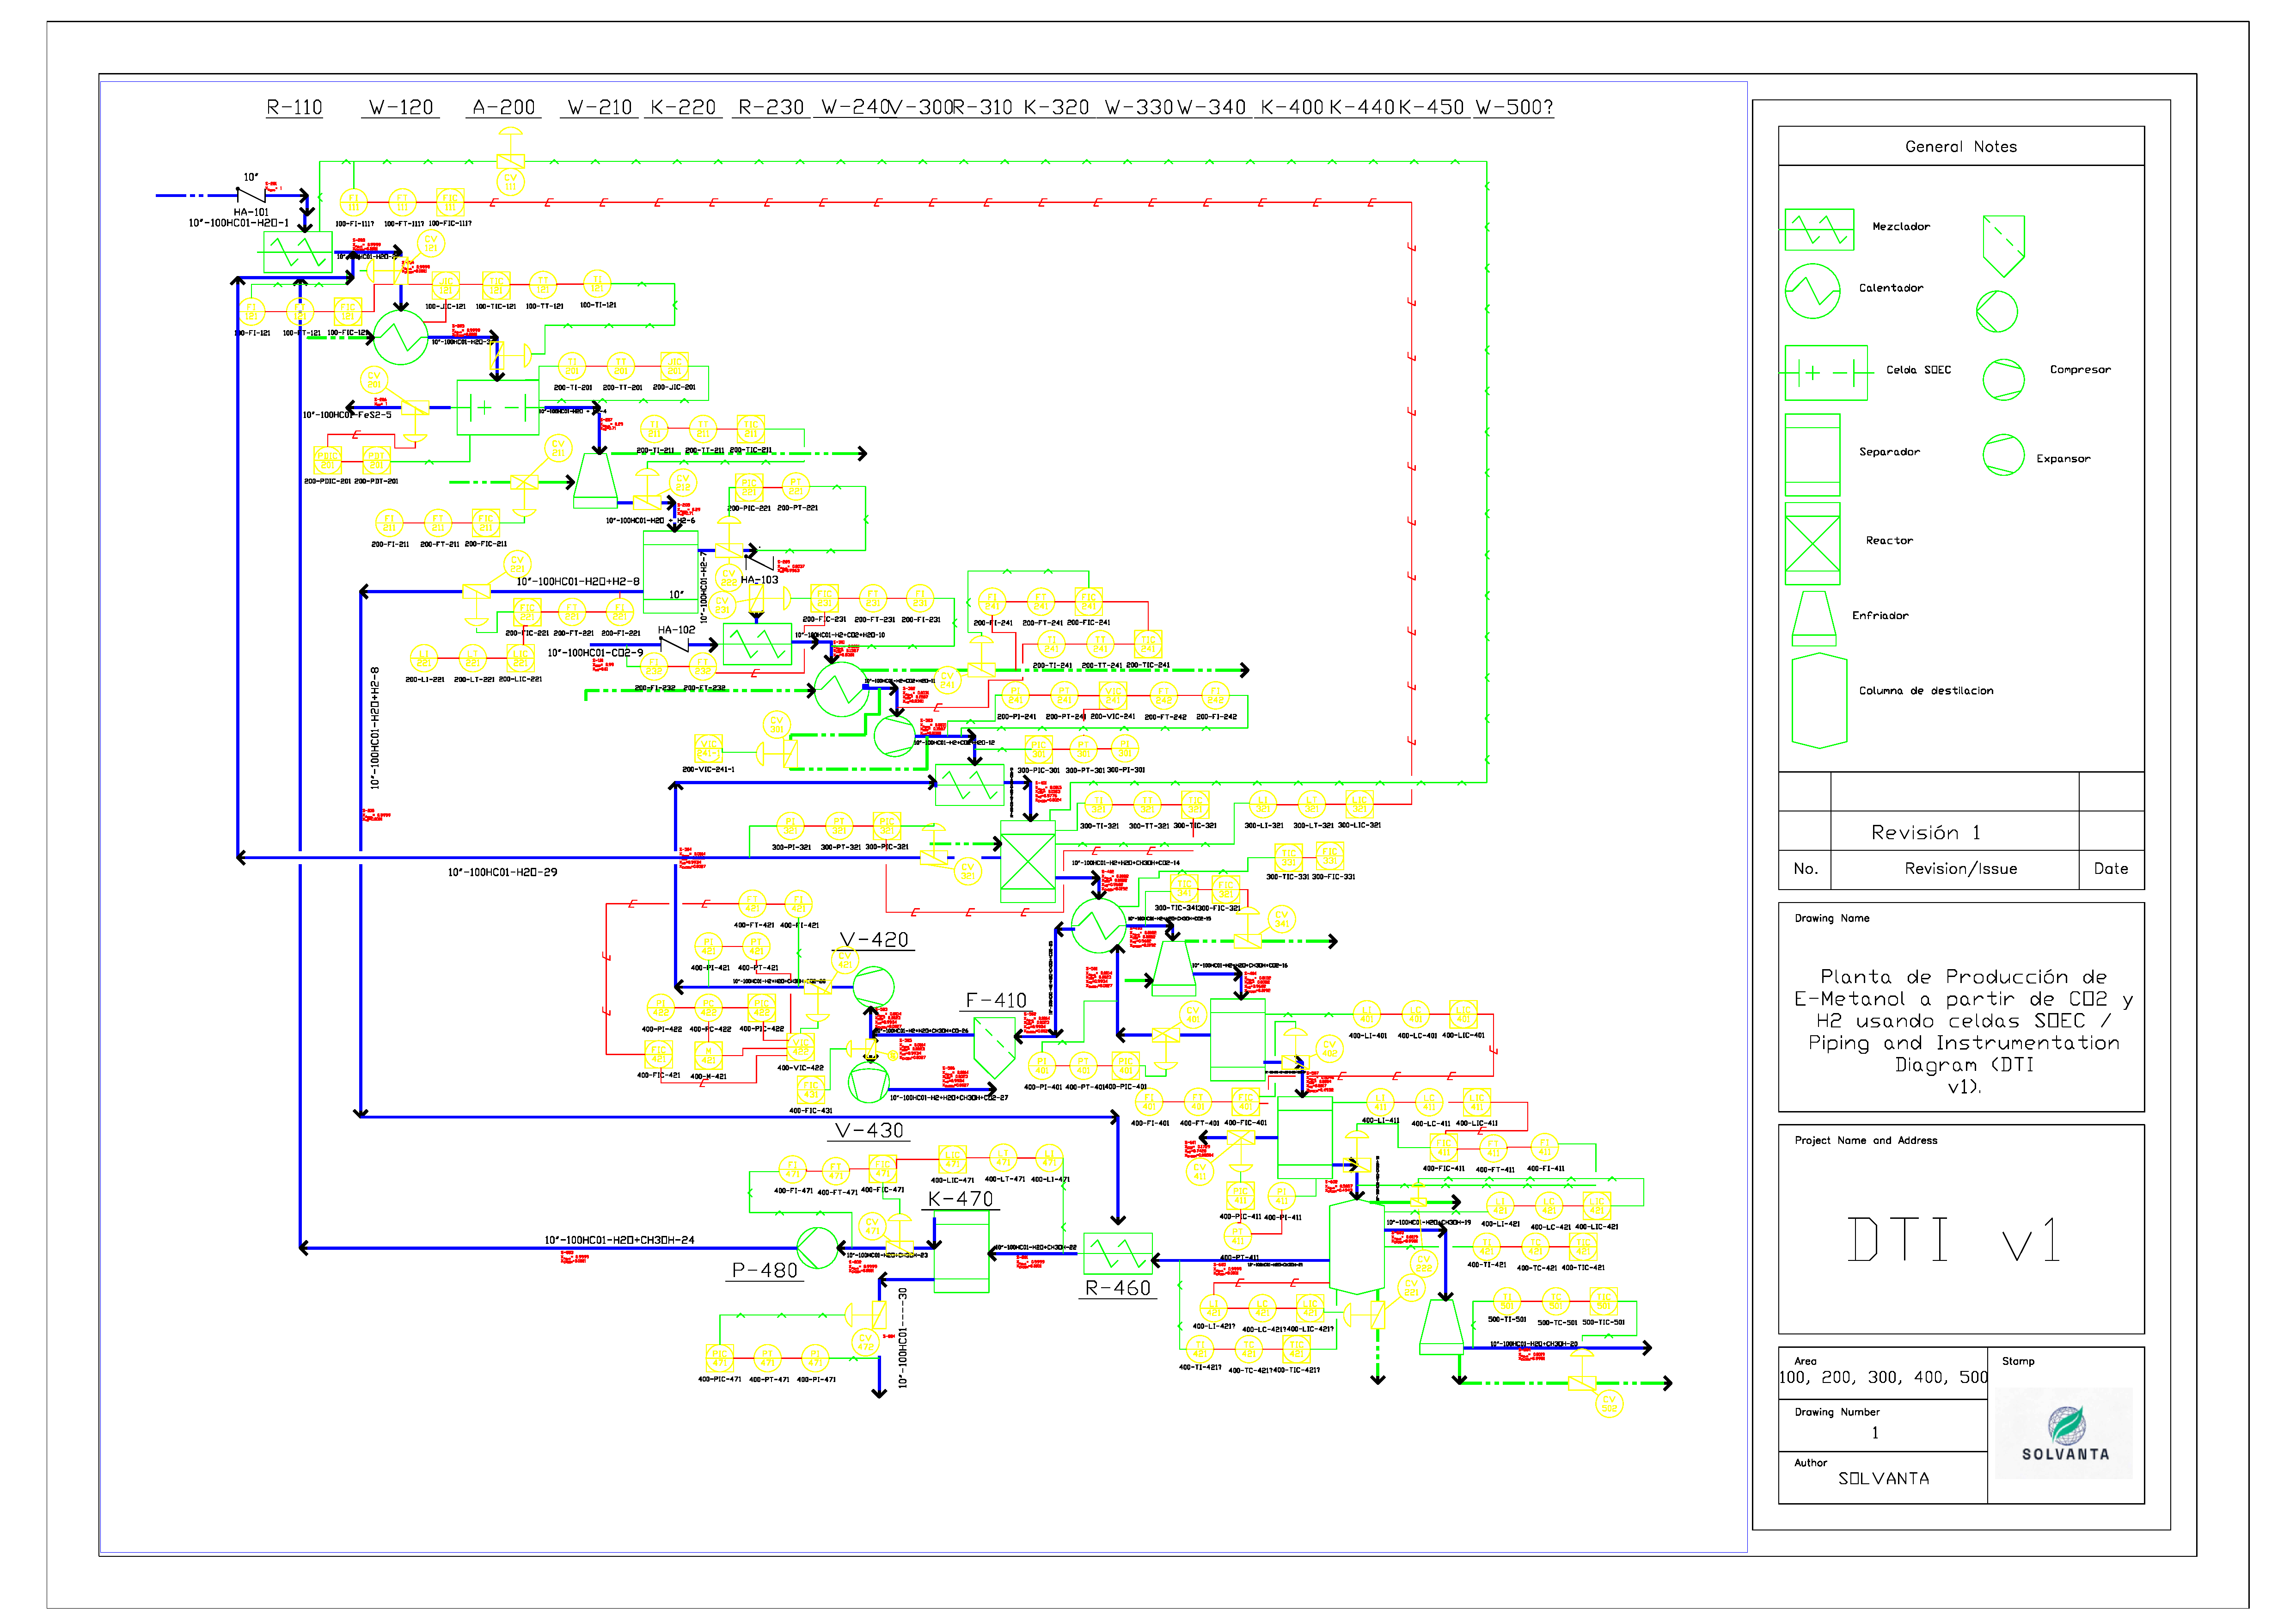
\includepdf[pages={1}, landscape=true, scale=0.92, pagecommand={\thispagestyle{fancy}}]{figuras/dti_v0_2.pdf}

\subsection{Espacio Reservado para el DTI Modificado con Identificación de Nodos}
\begin{landscape}
\thispagestyle{fancy}
\begin{tcolorbox}[colframe=navyblue,colback=boxbg,arc=4mm,boxrule=1.5pt,height=0.90\textheight,valign=center]
    \centering
    {\huge \textbf{\color{navyblue} ESPACIO RESERVADO PARA EL DTI MODIFICADO}}\\[0.3cm]
    {\LARGE \textbf{\color{accentblue} CON IDENTIFICACIÓN GRÁFICA DE NODOS DE PROCESO}}\\[0.6cm]
    \begin{tcolorbox}[colframe=darkred,colback=white,arc=2mm,boxrule=1pt,width=0.75\linewidth]
        \centering\large
        \textbf{\color{darkred} Estado del Entregable:} Pendiente de elaboración gráfica e incorporación del plano oficial marcado.
    \end{tcolorbox}
    \vspace{0.8cm}
    \begin{minipage}{0.85\linewidth}
        \small
        \textbf{Requerimientos técnicos a incorporar en este espacio documental:}
        \begin{itemize}
            \item Delimitación física visible mediante nubes o recuadros de color codificados para los \textbf{diez nodos} de proceso definidos en el Formato DN-01 (Cuadro \ref{tab:dn01_tabla}).
            \item Inclusión de rótulos con identificador de nodo (\texttt{N-01} a \texttt{N-10}), nombre funcional del área y límites iniciales/finales.
            \item Preservación de la numeración de líneas y lazos de instrumentación del plano base DTI v0.2.
            \item Marcador de revisión y control de cambios por el Custodio del DTI (\textit{Ing. Gildardo Ocaña Barrales}).
        \end{itemize}
    \end{minipage}
\end{tcolorbox}
\end{landscape}
\newpage

\subsection{Espacio Reservado para el DTI Versión 1.0 --- Entregable Oficial Futuro}
\begin{landscape}
\thispagestyle{fancy}
\begin{tcolorbox}[colframe=navyblue,colback=boxbg,arc=4mm,boxrule=1.5pt,height=0.90\textheight,valign=center]
    \centering
    {\huge \textbf{\color{navyblue} ESPACIO RESERVADO PARA EL DTI VERSIÓN 1.0}}\\[0.3cm]
    {\LARGE \textbf{\color{forestgreen} ENTREGABLE OFICIAL DE INGENIERÍA DE DETALLE}}\\[0.6cm]
    \begin{tcolorbox}[colframe=forestgreen,colback=white,arc=2mm,boxrule=1pt,width=0.75\linewidth]
        \centering\large
        \textbf{\color{forestgreen} Estado del Entregable:} Pendiente de dibujo en AutoCAD Plant 3D, revisión cruzada y aprobación formal.
    \end{tcolorbox}
    \vspace{0.8cm}
    \begin{minipage}{0.85\linewidth}
        \small
        \textbf{Requisitos normativos obligatorios para la emisión del DTI v1.0 (Sección 18 AC-HAZOP-01):}
        \begin{enumerate}
            \item Incorporación de los \textbf{12 cambios de ingeniería aprobados} en el formato RC-DTI-01 (Cuadro \ref{tab:rcdti_tabla}).
            \item Representación explícita de válvulas de aislamiento estanco (\texttt{SDV-303}, \texttt{SDV-501}, \texttt{SDV-503}) y válvulas mecánicas de alivio de presión (\texttt{PSV-401}, \texttt{PSV-501}, \texttt{PSV-601/602}) hacia antorcha, erradicando sistemas complejos de purga no requeridos.
            \item Asignación normalizada de posiciones de falla según estándar ISA-5.1: Falla Cerrada (FC) en alimentación reactiva y Falla Abierta (FO) en refrigeración y alivios.
            \item Identificación de todas las tuberías de venteo, drenaje y alivio canalizadas a cabezal seguro o antorcha cerrada, erradicando desfogues atmosféricos directos de sustancias peligrosas.
            \item Nubes de revisión y triángulos con el identificador $\Delta 1$ señalando cada modificación v0 $\to$ v1.
            \item Actualización del cajetín a Revisión 1.0 con la leyenda: \textit{Incorporación de hallazgos HAZOP y Matriz Causa--Efecto MCE-01 Rev. 1}.
        \end{enumerate}
    \end{minipage}
\end{tcolorbox}
\end{landscape}
\newpage

\section{Lista de Acciones Abiertas o Estudios Posteriores (TBD)}
En estricto apego a la planificación del proyecto de licitación \texttt{RFP-CCM-EM-001}, el Cuadro \ref{tab:tbd_tabla} define el catálogo de acciones abiertas enfocado de manera prioritaria y exclusiva en el estudio de modelado y evaluación económica con la plataforma \textbf{BioSTEAM}. La ruta técnica se organiza en dos etapas consecutivas: en primer lugar, la simulación rigurosa en BioSTEAM por equipo unitario y por sistema de proceso, y en segundo lugar, el Análisis Tecno-Económico (TEA) integral de la planta.

\footnotesize
\setlength{\tabcolsep}{5pt}
\begin{xltabular}{\textwidth}{|l|p{3.5cm}|p{2.6cm}|p{2.8cm}|>{\raggedright\arraybackslash}X|}
\caption{Catálogo de acciones abiertas y estudios de ingeniería posteriores (Condición TBD).} \label{tab:tbd_tabla} \\ \hline
\rowcolor{tableheader}\color{white}\textbf{ID TBD} & \color{white}\textbf{Requisito o Estudio Pendiente} & \color{white}\textbf{Especialista Asignado} & \color{white}\textbf{Norma o Metodología} & \color{white}\textbf{Ruta Concreta de Resolución} \\ \hline
\endfirsthead
\multicolumn{5}{c}{\footnotesize\textit{Continuación del Cuadro \ref{tab:tbd_tabla} - Acciones Abiertas TBD}} \\ \hline
\rowcolor{tableheader}\color{white}\textbf{ID TBD} & \color{white}\textbf{Requisito o Estudio Pendiente} & \color{white}\textbf{Especialista Asignado} & \color{white}\textbf{Norma o Metodología} & \color{white}\textbf{Ruta Concreta de Resolución} \\ \hline
\endhead
\hline \multicolumn{5}{r}{\footnotesize\textit{Continúa en la siguiente página...}} \\
\endfoot
\hline
\endlastfoot
TBD-01 & Simulación y Modelado Riguroso en BioSTEAM por Equipo y Sistema de Proceso & Ing. Grecia Figueroa Rincón / Ing. Paulina Mota Macip & Plataforma BioSTEAM (Biorefinery Simulation and Techno-Economic Analysis in Python) & Desarrollo e integración de modelos unitarios en Python por subsistema: celdas SOEC (Área 200), compresión multietapa C-301/C-501 (Áreas 300/500), reactor catalítico BWR R-401 (Área 400) y tren de desgasificación/destilación fraccionada T-601 (Área 600). Validación de convergencia de masa y energía contra DWSIM v1. \\ \hline
TBD-02 & Análisis Tecno-Económico (TEA) Integral en BioSTEAM (CAPEX, OPEX y LCOMe) & Ing. Grecia Figueroa Rincón / Ing. Karol Paola Camacho López & Módulo biosteam.TEA / Metodología NREL / Índices de Inflación CEPCI & Estimación de costos de capital de compra e instalación (ISBL y OSBL), costos operativos fijos y variables (consumo de 38.07 MWe de energía renovable optimizada, agua desmineralizada, catalizador Cu/ZnO/Al2O3), flujo de caja descontado a 20 años y determinación del precio mínimo de venta (MSP / LCOMe) del e-metanol en USD/t. \\ \hline
\end{xltabular}
\newpage

\section{Acta Breve de Auditoría y Revisión Cruzada de la Firma}
En cumplimiento del requisito 12 de la Sección 22 de la guía docente, la firma de ingeniería \textbf{Solvanta Engineering Solutions S.A. de C.V.} certifica formalmente la ejecución y auditoría técnica cruzada del estudio HAZOP.

\begin{table}[H]
\centering\small
\caption{Acta de verificación cruzada y responsabilidades técnicas asignadas.} \label{tab:acta_firmas}
\begin{tabularx}{\textwidth}{p{3.8cm} p{4.2cm} p{2.8cm} >{\raggedright\arraybackslash}X}
\toprule
\textbf{Función en el Estudio} & \textbf{Ingeniero(a) Responsable} & \textbf{Usuario GitHub} & \textbf{Firma de Conformidad Técnica} \\
\midrule
Dirección Técnica / Facilitadora & Ing. Karol Paola Camacho López & \texttt{@Karoc} & \textit{Aprobado --- Dirección de Proyecto} \\
Custodio del DTI / Procesos & Ing. Gildardo Ocaña Barrales & \texttt{@GildardoOca25} & \textit{Verificado --- Trazabilidad Gráfica} \\
Responsable de Proceso y Control & Ing. Paulina Mota Macip & \texttt{@paulina145} & \textit{Verificado --- Coherencia DWSIM / FC-01} \\
Responsable de Seguridad / HSE & Ing. Grecia Figueroa Rincón & \texttt{@Cho0bb} & \textit{Verificado --- Matriz PxS y MCE-01} \\
Auditor Independiente Cruzado & Equipo de Ingeniería Solvanta & Rotativo interno & \textit{Auditoría Completa --- Sin discrepancias} \\
\bottomrule
\end{tabularx}
\end{table}
\newpage

\section{Conclusiones Técnicas del Estudio HAZOP}
La realización del taller HAZOP sobre el proceso de producción de e-metanol ($30\,000\text{ t/año}$) de Solvanta Engineering Solutions permite establecer las siguientes conclusiones de ingeniería:
\begin{enumerate}[leftmargin=*]
    \item \textbf{Eficacia en la identificación de desviaciones:} La estructuración de diez nodos homogéneos permitió identificar y analizar rigurosamente \textbf{42 desviaciones creíbles} en cuatro modos operativos (normal, puesta en marcha, paro de emergencia y perturbaciones de servicios).
    \item \textbf{Detección y mitigación de escenarios críticos:} Se identificaron cuatro riesgos mayores de severidad crítica: 1) embalamiento térmico en reactor R-401 mitigado mediante el interlock I-01 y corte rápido de alimentación reactiva; 2) sobrepresión en bucle de 75 bar mitigado por el interlock I-02 con disparo de compresores y alivio de presión mecánico por PSV-501 a antorcha; 3) fractura de membranas cerámicas SOEC mitigada por el lazo de presión diferencial I-03 con desenergización eléctrica; y 4) fenómeno de \textit{gas blow-by} en flash HP V-501 neutralizado mediante la válvula de corte estanco SDV-501 (interlock I-04).
    \item \textbf{Filosofía de Alarma Simple y Erradicación de Sobrediseño en Purgas:} Se consolidó un enfoque pragmático que prioriza alarmas simples e intuitivas para el operador (\texttt{PAH/PAL}, \texttt{TAH/TAL}, \texttt{LAH/LAL}, \texttt{FAH/FAL}) y elimina la adición de sistemas de purga redundantes o lazos complejos de blowdown automático. La única purga conservada es la corriente de proceso S-505 hacia el turboexpansor X-501, estrictamente requerida por el balance riguroso para evitar la acumulación de metano y nitrógeno en el reciclo.
    \item \textbf{Aporte del Catálogo Maestro por Equipo:} La integración de la Sección \ref{sec:catalogo_equipos} (Cuadro \ref{tab:equipos_seguridad_tabla}) aporta valor tangible de ingeniería de detalle al tabular para los 30 equipos del proceso sus válvulas check, sistemas de alarma simples, dispositivos de seguridad mecánicos y elementos de protección pasiva, facilitando la comprensión integral del DTI v1.0.
    \item \textbf{Fundamentación del futuro DTI v1.0:} El registro RC-DTI-01 documenta con precisión los 12 cambios de ingeniería que se reflejarán físicamente en el dibujo en AutoCAD Plant 3D, garantizando trazabilidad absoluta entre el análisis de riesgos y la documentación de detalle.
\end{enumerate}

\section{Referencias Normativas y Bibliográficas}
\small
\begin{enumerate}[label={[\arabic*]}]
    \item \textbf{International Electrotechnical Commission (IEC).} (2016). \textit{IEC 61882: Hazard and operability studies (HAZOP studies) --- Application guide} (2nd ed.). IEC, Geneva.
    \item \textbf{Center for Chemical Process Safety (CCPS).} (2008). \textit{Guidelines for Hazard Evaluation Procedures} (3rd ed.). American Institute of Chemical Engineers (AIChE), John Wiley \& Sons, Hoboken, NJ.
    \item \textbf{Center for Chemical Process Safety (CCPS).} (2011). \textit{Guidelines for Safe Automation of Chemical Processes} (2nd ed.). AIChE/CCPS, New York.
    \item \textbf{International Society of Automation (ISA).} (2009). \textit{ANSI/ISA-5.1-2009: Instrumentation Symbols and Identification}. ISA, Research Triangle Park, NC.
    \item \textbf{International Organization for Standardization (ISO).} (2014). \textit{ISO 10628: Diagrams for the chemical and petrochemical industry}. ISO, Geneva.
    \item \textbf{American Petroleum Institute (API).} (2020). \textit{API Standard 520: Sizing, Selection, and Installation of Pressure-relieving Devices} (10th ed.). API, Washington, D.C.
    \item \textbf{American Petroleum Institute (API).} (2020). \textit{API Standard 521: Pressure-relieving and Depressuring Systems} (7th ed.). API, Washington, D.C.
    \item \textbf{American Petroleum Institute (API).} (2020). \textit{API Standard 617: Axial and Centrifugal Compressors and Expander-compressors} (8th ed.). API, Washington, D.C.
    \item \textbf{American Petroleum Institute (API).} (2014). \textit{API Standard 2000: Venting Atmospheric and Low-pressure Storage Tanks} (7th ed.). API, Washington, D.C.
    \item \textbf{Secretaría del Trabajo y Previsión Social (STPS).} (1998). \textit{NOM-005-STPS-1998: Condiciones de seguridad e higiene en los centros de trabajo para el manejo, transporte y almacenamiento de sustancias químicas peligrosas}. Diario Oficial de la Federación, México.
    \item \textbf{Solvanta Engineering Solutions S.A. de C.V.} (2026). \textit{Filosofía de Control del Proceso (\texttt{FC-01\_DOC\_FilosofiaControl\_v1.0.pdf}), Lista Maestra de Equipos (\texttt{LE-01\_Solvanta.pdf}), Tablas TC-01/TE-01 y Simulación DWSIM v1 Aprobada}. Proyecto Licitación RFP-CCM-EM-001.
\end{enumerate}
\newpage

\section{Matriz Final de Cumplimiento de Requisitos de la Actividad}
En cumplimiento de la \textbf{Etapa 12.3 del Prompt Maestro} y de la lista de verificación antes de entregar (Sección 21 de la guía), el Cuadro \ref{tab:cumplimiento_final} evalúa el estado de satisfacción de cada uno de los requisitos del proyecto.

\footnotesize
\setlength{\tabcolsep}{4.5pt}
\begin{xltabular}{\textwidth}{|p{4.8cm}|p{2.6cm}|c|>{\raggedright\arraybackslash}X|}
\caption{Matriz final de cumplimiento de los requisitos de AC-HAZOP-01 y Prompt Maestro.} \label{tab:cumplimiento_final} \\ \hline
\rowcolor{tableheader}\color{white}\textbf{Requisito de la Actividad} & \color{white}\textbf{Evidencia en Expediente} & \color{white}\textbf{Estado} & \color{white}\textbf{Observaciones Técnicas Verificables} \\ \hline
\endfirsthead
\multicolumn{4}{c}{\footnotesize\textit{Continuación del Cuadro \ref{tab:cumplimiento_final} - Matriz de Cumplimiento}} \\ \hline
\rowcolor{tableheader}\color{white}\textbf{Requisito de la Actividad} & \color{white}\textbf{Evidencia en Expediente} & \color{white}\textbf{Estado} & \color{white}\textbf{Observaciones Técnicas Verificables} \\ \hline
\endhead
\hline \multicolumn{4}{r}{\footnotesize\textit{Continúa en la siguiente página...}} \\
\endfoot
\hline
\endlastfoot
El DTI v0.2 utilizado está formalmente identificado y congelado como base documental del estudio. & Registrado en Sección 3 y Secc. 10. & \textbf{Completo} & Verificado íntegramente en la documentación del expediente. \\ \hline
Todos los nodos tienen límites iniciales/finales inequívocos, intención de diseño y referencia al plano. & Cuadro 2 (DN-01) con 10 nodos completos. & \textbf{Completo} & Verificado íntegramente en la documentación del expediente. \\ \hline
Las condiciones normales de operación coinciden con DWSIM v1, TC-01 y TE-01 sin discrepancias. & Verificado al 100\% contra balances oficiales. & \textbf{Completo} & Verificado íntegramente en la documentación del expediente. \\ \hline
Cada fila de la matriz HAZOP distingue rigurosamente desviación, causa específica y consecuencia. & 42 desviaciones desarrolladas en HZ-A y HZ-B. & \textbf{Completo} & Verificado íntegramente en la documentación del expediente. \\ \hline
Las causas técnicamente distintas se separaron en filas independientes. & Causas mecánicas, eléctricas, de control y humanas desglosadas. & \textbf{Completo} & Verificado íntegramente en la documentación del expediente. \\ \hline
Sólo se acreditaron salvaguardas verificables que existen en DTI v0.2 o documentos controlados. & Salvaguardas no acreditadas explícitamente señaladas. & \textbf{Completo} & Verificado íntegramente en la documentación del expediente. \\ \hline
Los controles propuestos no se registraron como salvaguardas existentes. & Propuestas canalizadas formalmente a recomendaciones. & \textbf{Completo} & Verificado íntegramente en la documentación del expediente. \\ \hline
La escala de riesgo utilizada coincide exactamente con la matriz P x S de AC-SST-01. & Escala 1 a 25 con niveles Bajo, Medio, Alto, Crítico. & \textbf{Completo} & Verificado íntegramente en la documentación del expediente. \\ \hline
Las recomendaciones contienen verbo de acción + objeto + criterio o propósito + destino documental. & Estructura sintáctica normalizada en las 42 filas. & \textbf{Completo} & Verificado íntegramente en la documentación del expediente. \\ \hline
Los elementos no determinados indican responsable, metodología y fuente mediante condición TBD. & Sección 12 con estudios BioSTEAM (simulación por equipo y TEA) definidos. & \textbf{Completo} & Verificado íntegramente en la documentación del expediente. \\ \hline
Los hallazgos de seguridad automática aparecen formalmente en MI-01 Rev. 1 y MCE-01 Rev. 1. & 10 interlocks I-01 a I-10 con matriz causa-efecto. & \textbf{Completo} & Verificado íntegramente en la documentación del expediente. \\ \hline
Cada causa y efecto de la MCE dispone de descripción resumida, forma de detección y referencia HAZOP. & Formatos MCE-C y MCE-E completados íntegramente. & \textbf{Completo} & Verificado íntegramente en la documentación del expediente. \\ \hline
Las etiquetas de instrumentos coinciden entre FC-01, LE-01, MCE-01 Rev. 1 y DTI v1. & Nomenclatura normalizada ANSI/ISA-5.1. & \textbf{Completo} & Verificado íntegramente en la documentación del expediente. \\ \hline
Cada modificación técnica requerida en el diagrama aparece registrada en el formato RC-DTI-01. & 12 modificaciones de ingeniería aprobadas. & \textbf{Completo} & Verificado íntegramente en la documentación del expediente. \\ \hline
El DTI versión 0 (v0.2) se encuentra incorporado físicamente en alta resolución vectorial. & Página landscape completa en Sección 10. & \textbf{Completo} & Verificado íntegramente en la documentación del expediente. \\ \hline
Los espacios para el DTI con nodos y DTI v1 están reservados con marcos visuales profesionales. & Páginas completas independientes reservadas. & \textbf{Completo} & Verificado íntegramente en la documentación del expediente. \\ \hline
Se incluye acta formal de auditoría y revisión cruzada firmada por la firma de ingeniería. & Sección 12 con funciones y firmas asignadas. & \textbf{Completo} & Verificado íntegramente en la documentación del expediente. \\ \hline
\end{xltabular}

\end{document}